\documentclass{vorkurs}
\usepackage[utf8]{inputenc}
\usepackage[T1]{fontenc}

\usepackage{xspace}
\usepackage[pass]{geometry}
\usepackage{tikz}
\usetikzlibrary{arrows,decorations.pathmorphing,decorations.footprints,fadings,calc,trees,mindmap,shadows,decorations.text,patterns,positioning,shapes,matrix,fit}
\usepackage{enumitem}
\usepackage{url}
\usepackage[pdftex,bookmarks=true,bookmarksnumbered=true,bookmarksopen=true,colorlinks=true,filecolor=black,
    linkcolor=red,urlcolor=blue,plainpages=false,pdfpagelabels,citecolor=black,
    pdftitle={Programmiervorkurs der Fachschaft
    MathPhys},setpagesize=false,pdfauthor={Axel Wagner}]{hyperref}

\newcommand{\swname}[1]{\texttt{#1}\xspace}
\newcommand{\Cpp}{\swname{C++}}
\newcommand{\file}[1]{\texttt{#1}\xspace}
\newcommand{\param}[1]{\texttt{#1}\xspace}

\begin{document}

Um Lesbarkeit zu gewährleisten, nutzt dieses Schriftstück das generische
Femininum.

Soweit personenbezogene Bezeichnungen in weiblicher Form aufgeführt sind,
beziehen sie sich auf alle Geschlechter in gleicher Weise.

\clearpage

\chapter*{Vorwort}
\pagestyle{empty}

Vorliegend ist der Programmier-Einführungskurs der Fachschaft MathPhys.

Gedacht ist dieser für Menschen, die ihren Computer bisher eher zum Spielen,
als zum Arbeiten benutzt haben, die vielleicht noch nicht wissen, dass es
andere Betriebssysteme als DasBekannteVonDerRedmonderFirma™ oder
DasMitDemApfelDrauf (You probably never heard of it) gibt, geschweige denn,
dass sie mal eine Shell benutzt haben - oder auch nur wissen, was zur Hölle das
sein soll.  Die schon mal gehört haben, dass man „Programmieren“ kann, sich
darunter aber einen magischen Prozess vorstellen, der nur Eingeweihte
beherrschen und von dem man eigentlich lieber die Finger lässt, wenn man nicht
will, dass einem der Computer um die Ohren fliegt.  Kurzum: Dieser Kurs richtet
sich an blutigste Anfängerinnen.

Wir wollen zeigen, dass Programmieren eigentlich gar nicht so schwer ist, dass
eine Shell ein mächtiges Werkzeug ist und dass einem der Computer eigentlich
viel mehr Spaß bringt, wenn man mit dem nötigen Spieltrieb herangeht.  Am Ende
dieses Kurses sollte die Angst vor dem Computer verflogen sein. Ihr solltet
gesehen haben, dass es keinen Grund gibt, ewig zu rätseln, ob ein Algorithmus
nun korrekt ist und was die richtige Syntax für eine Operation ist, statt
einfach etwas hinzuschreiben und zu sehen, ob es kompiliert.  Die wichtigste
Kompetenz, die wir euch vermitteln wollen ist, programmieren zu lernen, also zu
wissen, wie man eine Fehlermeldung liest, wo man bei Wissenslücken nachschauen
kann und wen man fragen kann, wenn man mal nicht weiter weiß.

Um diese Ziele zu erreichen, haben wir den Kurs aufgeteilt in viele kleine
Lektionen. Jede Lektion stellt im Wesentlichen eine abgeschlossene Einheit da,
die eigenständig (mit bedarfsorientierter Hilfestellung) bearbeitet werden
sollen. Primär geht es dabei nicht um den dargestellten Inhalt, sondern darum,
mit diesem herumzuspielen und selbst die cornercases zu entdecken.
Insbesondere solltet ihr die Lektionen also \emph{nicht} unter künstlichem
Zeitdruck bearbeiten, das Ziel ist nicht, jede Lektion bearbeitet zu haben,
sondern jede Lektion entdeckt zu haben.  Selbstverantwortliches Lernen ist
tragender Gedanke des Kurses und sollte entsprechend ernst genommen werden;
entscheidet selbst, wie viel Zeit ihr in welche Lektionen stecken wollt.

Jede Lektion gliedert sich wiederum in drei Teile:
\begin{enumerate}
    \item Ein theoretischer, in dem ein Unterbau für die Lektion gegeben werden
        soll.  Ein tiefes Verständnis sollte für die Bearbeitung der Lektion
        nicht notwendig sein, es geht mehr darum, dass sich ein grober
        Wiedererkennungseffekt einstellt, wenn die theoretischen Kenntnisse im
        nächsten Teil vertieft werden.

        Wenn du einen eher passiven Lernstil pflegst, kannst du dir hier auch
        einen Tutor zur Seite stellen lassen, der dich kurz in das Thema
        einführt.
    \item Dem Theorieteil schließt sich der Praxisteil an.
        Hier soll selbstständig das eben hoffentlich oberflächlich verstandene
        in einer kurzen Fingerübung angewendet werden.

        Bei Fragen kann man aber natürlich auch hier einen Tutor zu Rate
        ziehen.
    \item Zuletzt steht dann ein Spielteil. Hier soll mit das Gelernte vertieft und bespielt werden.
        Tiefer gehende Informationen werden vermittelt und Möglichkeiten, mit
        dem Code zu interagieren aufgezeigt.

        Von diesem Teil sollte man sich am Wenigsten aufhalten, verunsichern
        oder deprimieren lassen.
\end{enumerate}

Als Sprache für den Kurs haben wir \Cpp gewählt.  Diese Sprache stellt
vergleichsweise hohe Anforderungen an Anfänger, da sie relativ maschinennah
ist, nicht „garbage-collected“ ist (was auch immer das heißen mag) und
high-level Konstrukte wie Listen oder Hashtables keine Repräsentation in der
Syntax haben.  Es muss also viel manuell gemacht werden und das Ganze in einer
verhältnismäßig strikten Syntax.

Der Grund, aus dem wir trotzdem \Cpp gewählt haben, ist, dass in den
Anfängervorlesungen der Universität Heidelberg \Cpp verwendet wird und wir euch
die Verwirrung ersparen wollen, direkt zu Beginn des Lernprozesses mit zwei
verschiedenen Sprachen konfrontiert zu werden.  Ausserdem gibt es uns
Gelegenheit, direkt wichtige Sprachidiome einzuführen, den Aufprall des ersten
Kontaktes abzufedern und durch Demonstration sprachspezifischer Hilfswerkzeuge
(wie zum Beispiel dem gdb) zu verhindern, dass ihr bei typischen Problemen der
Sprache im späteren Studienverlauf in Verzweifelung versinkt.

Der gesamte Kurs ist aufgeteilt in mehrere Kapitel. Dies dient dem Zweck,
verschiedenste Bedürfnisse und Lerntempi zu befriedigen.  Wer sich ganz auf die
Grundlagen konzentrieren und sich mit diesen intensiv auseinandersetzen möchte,
findet in den ersten Kapiteln Material, spielerisch die Sprache zu entdecken.
Wer sich im ersten Kapitel relativ wohl fühlt, ist bereits bestens auf die
Einführung in die praktische Informatik vorbereitet.  Wer schneller lernt, oder
einen tieferen Einblick wünscht, findet in späteren Kapiteln genug Material, um
sich trotzdem für zwei Wochen zu beschäftigen und voll in die Sprache
einzusteigen.

Insgesamt sollte noch einmal betont werden, dass der Selbstanspruch, den
gesamten Kurs in vorgegebener Zeit durchzuarbeiten, dem Lernprozess schadet.
Der Kurs wird nicht benotet, gibt keine Creditpoints und ihr könnt ihn auch
nicht auf eurer Bewerbung angeben - für wen hetzt ihr euch also ab?

\tableofcontents

\chapter{Die Basics}
\pagestyle{empty}

Im Ersten Kapitel werden wir die Grundlagen der Programmierung lernen.

Wir werden rausfinden, was ein Compiler ist, wie ein Programm abläuft und wie
man es startet. Wir werden Benutzereingaben verarbeiten und Ausgaben an die
Nutzerin geben. Wir lassen den Computer Rechnungen für uns anstellen und
lernen, was der Kontrollfluß ist - und wie man ihn beeinflusst. Zuletzt werden
wir Arrays kennenlernen und unser erstes nützliches Progamm schreiben.

\lesson{Hello world}

Die erste Lektion beschäftigt sich alleine mit der Frage, was eigentlich eine
Programmiersprache überhaupt ist und wie wir den Computer dazu bringen können,
daraus etwas zu machen, was er ausführen kann.  In guter alter
Programmiertradition tun wir das an dem simpelsten aller Programme: Einem, was
einfach nur ein „Hallo Welt!“ ausgibt.

Wie bringen wir also den Computer dazu, diese Ausgabe zu generieren? Dass er
keine natürliche Sprache versteht, sollte klar sein - intern besteht er aus
lauter Transistoren (wenn ihr nicht wisst, was das ist, denkt an winzige
Schalter), die nur die Zustände „an“ und „aus“ kennen, wir müssen also die
Anweisung „gebe Hallo Welt aus“ in ein Format übersetzen, was nur „an“ und
„aus“ benutzt.

Früher wurde genau dies benutzt - meistens über Lochkarten, die vom Computer
gelesen wurden, „ein Loch“ war dann zum Beispiel ein „an“ und „kein Loch“ war
„aus“, so wurde dann das Programm in Reihen angeordnet und jede Reihe entsprach
einem Befehl oder einem Parameter für diesen Befehl.  Dieses Format nennt sich
„Maschinensprache“ und ist immer noch das, was wir heute dem Computer
übergeben, nur, dass wir keine Lochkarten mehr benutzen, sondern Dateien, in
denen lange Ströme von codierten 0en und 1en stehen.

Nun kann man sich vorstellen, dass es ganz schön anstrengend ist, ein
umfangreiches Programm in 0en und 1en zu beschreiben. Deswegen benutzt man
heutzutage so genannte Hochsprachen, um Programme zu beschreiben. Wir
beschreiben also den Programmablauf in einer von Menschen lesbaren und
verstehbaren Sprache -- wir benutzen hier \Cpp.  Die Programmbeschreibung in
\Cpp legen wir dabei in einer Textdatei ab, meistens hat diese die Endung
\texttt{.cpp}.

Diese Beschreibung des Programms übergeben wir dann an einen \emph{Compiler},
der daraus dann Maschinencode generiert, den wir wiederum dem Computer zur
Ausführung geben können.  Der Compiler für \Cpp, den wir in diesem Kurs
benutzen wollen, heißt \texttt{g++}.

Dem Compiler übergeben wir die zu kompilierende Datei als Parameter, indem wir
sie im Terminal dahinter schreiben:
\begin{center}
\texttt{g++ zuKompilierendeDatei.cpp}
\end{center}
Wir können zusätzlich den Namen der Ausgabedatei festlegen, indem wir vor diese
ein \texttt{-o} (o für output) schreiben:
\begin{center}
\texttt{g++ -o outputDatei zuKompilierendeDatei.cpp}
\end{center}

Nachdem \texttt{g++} uns also ein Maschinencodefile \texttt{outputDatei}
erzeugt hat, können wir es zur Ausführung bringen. Wir tun das, indem wir in
einem Terminal
\begin{center}
	\texttt{./outputDatei}
\end{center}
eingeben, also einen Punkt, ein Slash und dann den Dateinamen.

Zur besseren Übersichtlichkeit hier der ganze Vorgang noch mal in einem
Diagramm:

% TODO: Buttugly, but well...
\begin{center}
    \resizebox{\textwidth}{!}{
        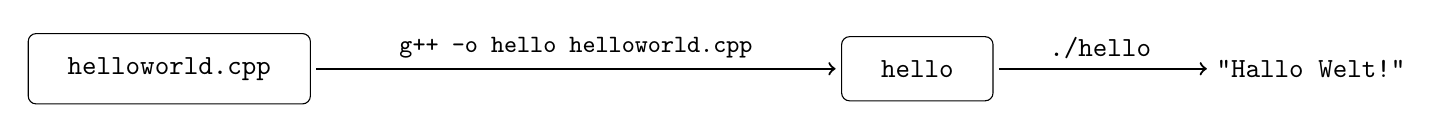
\begin{tikzpicture}
            \node (nHelloWorldCpp) [ shape=rectangle, rounded corners = 0.1cm, draw=black, inner xsep=0.5cm, inner ysep = 0.3cm ] {\texttt{helloworld.cpp}};
            \node (nHello) [ right of = nHelloWorldCpp, node distance = 9.5cm, shape=rectangle, rounded corners = 0.1cm, draw = black, inner xsep = 0.5cm, inner ysep = 0.3cm ] {\texttt{hello}};
            \draw [->, thick, shorten >= 2pt, shorten <= 2pt ] (nHelloWorldCpp) -- (nHello) node [ midway, above, font = \small ] { \texttt{g++ -o hello helloworld.cpp}} ;
            \node (nOutput) [ right of = nHello, node distance = 5cm, shape=rectangle ] {\texttt{"Hallo Welt!"}};
            \draw [->, thick, shorten <= 2pt] (nHello) -- (nOutput) node [ midway, above ] {\texttt{./hello}};
        \end{tikzpicture}
    }
\end{center}

\textbf{Praxis:}
\begin{enumerate}
	\item Öffnet ein Terminal, ihr findet dies in den Anwendungen (oben rechts)
		unter „Systemwerkzeuge“
    \item Wechselt in das Verzeichnis \texttt{vorkurs/lektion01}, indem ihr
		\texttt{cd vorkurs/lektion01}\footnote{was dieser Befehl genau tut und wie er funktioniert, erfahrt ihr in Lektion 2} eingebt und enter drückt.
    \item In diesem Verzeichnis liegt eine Datei \texttt{helloworld.cpp}.
        Benutzt \texttt{g++}, um diese zu einer Datei \texttt{hello} zu
        kompilieren. Orientiert euch dazu an den Befehlen von oben.
    \item Führt die Datei \texttt{hello} aus.
\end{enumerate}

\inputcpp{helloworld.cpp}

\textbf{Spiel:}

Ihr könnt nun versuchen, den Quellcode selbst zu verändern und damit ein wenig
herumzuspielen. Öffnet dazu einen Editor (in den Anwendungen findet ihr z.B.
unter „Zubehör“ den Editor gedit) und öffnet die Datei
\texttt{vorkurs/lektion01/helloworld.cpp}\footnote{entweder mittels
"Datei/Öffnen" in gedit oder über das Terminal mittels \texttt{gedit
helloworld.cpp}}. Denkt daran, nach jeder Änderung die Datei zu speichern und
im Terminal neu zu kompilieren und auszuführen.

Dinge, die ihr ausprobieren könntet sind zum Beispiel:
\begin{enumerate}
    \item Was passiert, wenn ihr „Hello world!“ in etwas anderes ändert?
    \item Was passiert, wenn ihr die erste Zeile löscht (der Originalquellcode
        ist in diesem pdf enthalten, ihr könnt sie also später wieder
        herstellen)?
    \item Was passiert, wenn ihr das „\verb|<< std::endl|“ löscht?
    \item Wie könnte man mehrere Sätze ausgeben? Wie könnte man mehrere Zeilen
        ausgeben?
\end{enumerate}

\lesson{Die Shell}

Wenn ihr bisher nur mit Windows oder Mac gearbeitet habt, habt ihr
wahrscheinlich in der letzten Lektion nebenbei etwas neues Kennen gelernt: Die
Shell.

Auch wenn sich unter Linux zunehmend Desktopumgebungen, wie man sie von
kommerziellen Betriebssystemen kennt verbreiten, bleibt die Shell immer noch das
Mittel der Wahl, wenn man sich mit dem System auseinander setzen, oder auch
allgemein arbeiten will. Wir erachten zumindest die Shell als wichtig genug, um
euch direkt zu beginn damit zu konfrontieren.

Wann immer ihr über das Anwendungsmenü ein Terminal startet, wird dort drin
automatisch auch eine shell gestartet. Die beiden Konzepte sind tatsächlich so
eng miteinander verknüpft, dass ihr euch um die Unterschiede erst einmal keine
Gedanken machen müsst - wann immer ihr Shell oder Terminal hört, denkt einfach
an das schwarze Fenster mit dem Text. Das ist auch das wesentliche Merkmal der
Shell, sie ist ein Textbasiertes interface zu eurem Computer. Ihr gebt Befehle
ein, sie gibt euch Text zurück und auf diese Weise könnt ihr eigentlich alles
machen, was ihr sonst gewohnterweise mit der Maus und grafischen Oberflächen
tun würdet.

Wenn die Shell auf eure Befehle wartet, zeigt sie euch den so genannten
\emph{Prompt} an. Er enthält unter anderem euren Nutzernamen und das aktuelle
Verzeichnis (\verb|~| steht dabei für euer Nutzerverzeichnis, ein spezieller
Ordner, der eurem Account zugeordnet ist und in dem ihr alle Rechte besitzt).

Wenn ihr in ein anderes Verzeichnis wechseln wollt, könnt ihr das (wie ihr
bereits in der ersten Lektion gelernt habt) mit dem Befehl \texttt{cd} tun,
gefolgt von dem Namen des Verzeichnis. Um zurück zu gehen, könnt ihr das
spezielle Verzeichnis \texttt{..} (also zwei Punkte) angeben, welches für das
nächst höher liegende Verzeichnis steht. Wenn ihr euch den Inhalt des
Verzeichnisses anschauen wollt, könnt ihr dafür den Befehl \texttt{ls}
benutzen. Um herauszufinden, in welchem Verzeichnis ihr euch befindet, könnt
ihr \texttt{pwd} nutzen, zum Kompilieren von C++-Programmen habt ihr den Befehl
\texttt{g++} kennengelernt. Solltet ihr Hilfe zu irgendeinem Befehl benötigen,
könnt ihr den Befehl \texttt{man} (für „Manual“) geben, gefolgt von dem Befehl,
zu dem ihr Hilfe braucht (über \texttt{man} werden wir später noch
ausführlicher reden).

\textbf{Praxis:}
\begin{enumerate}
    \item Öffnet ein Terminal und gebt die folgenden Befehle ein:
    \inputshell{basics.sh}
\end{enumerate}

\textbf{Spiel:}
\begin{enumerate}
    \item Versucht selbst, euer Nutzerverzeichnis (\emph{home}) zu navigieren.
        Wie viele Lektionen hat der Vorkurs?
    \item Was passiert, wenn ihr euer Homeverzeichnis verlasst (\texttt{cd ..}
        während ihr darin seid)?
    \item Versucht in der manpage von ls (\texttt{man ls}) zu stöbern und die
        verschiedenen Parameter, mit denen ihr das Verhalten steuern könnt zu
        erforschen. Findet ihr heraus, wie ihr ein longlisting anzeigen lässt,
        in dem unter anderem auch die Dateigröße zu jeder Datei steht?
\end{enumerate}

\lesson{Input und Output}

Nachdem wir ein bisschen Vertrauen in die shell entwickelt haben und zumindest
bereits unser erstes Programm kompiliert, wollen wir nun etwas spannendere
Dinge tun. Nach wie vor müsst ihr nicht jede Zeile eures Programmes verstehen.
Sollte euch bei einer bestimmten Zeile trotzdem interessieren, was genau sie
tut, versucht doch eventuell sie zu entfernen, das Programm zu kompilieren und
schaut, was sich ändert.

Wir wollen uns nun mit grundlegendem input und output vertraut machen, denn
erst wenn euer Programm mit einer Benutzerin interagiert, wird es wirklich
nützlich. Wir haben in der ersten Lektion bereits \texttt{cout} (für
\emph{console out}) kennengelernt, um Dinge auszugeben. Nun nutzen wir
\texttt{cin}, um Eingaben des Benutzers entgegen zu nehmen. Jedes Programm
unter Linux (und übrigens auch Mac OS oder Windows) kann auf diese Weise
Eingaben von der Nutzerin entgegen nehmen und Ausgaben liefern. Das ist auch
der Grund, warum die Konsole so wichtig ist und es viele Dinge gibt, die nur
mittels einer Konsole gelöst werden können: Während es viele Stunden dauert,
ein grafisches Interface zu programmieren, über die man mit dem Programm mit
der Maus kommunizieren kann, kann praktisch jeder ein textbasiertes
Konsoleninterface schreiben. Linux ist ein Ökosystem mit einer gewaltigen
Anzahl tools für jeden denkbaren Zweck und bei den meisten haben die Autorinnen
sich nicht die Mühe gemacht, extra eine grafische Oberfläche zu entwickeln.

Nun aber direkt zur Praxis:

\textbf{Praxis:}
\begin{enumerate}
    \item Öffnet die Datei \texttt{vorkurs/lektion03/helloyou.cpp} in eurem Texteditor
    \item Öffnet ein Terminal und wechselt in das Verzeichnis \texttt{vorkurs/lektion3}
    \item Kompiliert im Terminal die Datei (\texttt{g++ -o helloyou
        helloyou.cpp}) und führt sie aus (\texttt{./helloyou})
    \item Versucht verschiedene Eingaben an das Programm und beobachtet, was passiert
\end{enumerate}

\inputcpp{helloyou.cpp}

\textbf{Spiel:}

\begin{enumerate}
    \item Versucht, zu verstehen, was die einzelnen Teile des Programms tun. An
        welcher Stelle erfolgt die Eingabe? Was passiert dann damit?
    \item Erweitert das Programm um eigene Fragen und Ausgaben. Vergesst nicht,
        dass ihr das Programm nach jeder Änderung neu kompilieren und testen
        müsst.
\end{enumerate}

\lesson{Fehlermeldungen und häufige Fehler}

Wenn ihr in den vergangen Lektionen ein bisschen herumprobiert habt, wird es
euch sicher das ein oder andere mal passiert sein, dass euch der Compiler statt
eines funktionierenden Programms eine Riesenmenge Fehlermeldungen ausgespuckt
hat und ihr einen Schreck bekamt und schon dachtet, ihr hättet alles kaputt
gemacht.

\texttt{g++} ist leider bei Fehlermeldungen immer sehr ausführlich und gibt
euch lieber viel zu viel, als viel zu wenig aus. Das kann im ersten Blick ein
bisschen überwältigend wirken, aber wenn man einmal gelernt hat, wie die
Fehlermeldungen am Besten zu lesen sind, ist das alles gar nicht mehr so
schlimm.

Wir schieben deswegen eine Lektion über häufige Fehlerquellen ein und wie man
Fehlermeldungen von \texttt{g++} liest, um möglichst schnell die Ursache des
Fehlers zu finden.

Nehmen wir z.B. mal folgendes Programm:

\inputcpp{fehler1.cpp}

Wenn wir versuchen, dieses zu kompilieren, gibt uns \texttt{g++} folgendes aus:

\begin{textcode*}{label=g++ -o fehler1 fehler1.cpp}
fehler1.cpp: In function 'int main()':
fehler1.cpp:2:5: error: 'cout' is not a member of 'std'
fehler1.cpp:2:35: error: 'endl' is not a member of 'std'
\end{textcode*}

Wenn wir diese Fehlermeldung verstehen wollen, fangen wir immer ganz oben an,
egal wie viel Text uns der Compiler ausspucken mag. In diesem Fall sagt uns die
erste Zeile, in welcher Datei (\texttt{fehler1.cpp}) der Fehler aufgetreten ist
und in welcher Funktion (\texttt{int main()}). Die beiden Zeilen
danach sind sogar noch spezifischer: Sie enthalten zu Beginn den Dateinamen,
dann einen Doppelpunkt, gefolgt von einer Zeilennummer, gefolgt von einer
Spaltennummer. Das gibt euch ganz genau die Stelle an, an der der Compiler
etwas an eurem Code zu bemängeln hat. In diesen Fall ist, was der Compiler
bemängelt, dass \texttt{cout} bzw. \texttt{endl} nicht in \texttt{std} sind.
Was genau \texttt{std} bedeutet muss uns nicht interessieren, aber der Rest
sagt uns (mit ein bisschen Erfahrung) dass wir die Definition von \texttt{cout}
und \texttt{endl} nicht haben - was nicht weiter verwunderlich ist, denn diese
beiden Dinge werden in der Datei \texttt{iostream} definiert, die wir früher
immer includiert haben.

Damit wissen wir jetzt auch (endlich) was das \mint{c++}|#include <iostream>|
zu bedeuten hatte. Offenbar brauchen wir das, wenn wir Konsolen input und
output machen wollen, da es die Definitionen von \texttt{cout}, \texttt{cin},
\texttt{endl} und ähnlichem enthält.

Der nächste sehr häufig vorkommende Fehler ist subtiler:

\inputcpp{fehler2.cpp}

Wenn wir versuchen, dies zu kompilieren, bekommen wir vom Compiler
entgegengespuckt:

\begin{textcode*}{label=g++ -o fehler2 fehler2.cpp}
fehler2.cpp: In function 'int main()':
fehler2.cpp:5:1: error: expected ';' before '}' token
\end{textcode*}

Wiederum sagt uns die erste Zeile, in welcher Datei und Funktion der Fehler
aufgetreten ist. Die zweite Zeile sagt uns wo, nämlich in Zeile 5, direkt am
Anfang. Die Beschwerde des Compilers ist, dass er ein Semikolon erwartet hat,
aber eine geschlossene geschweifte Klammer gefunden hat. Der Grund dafür ist,
dass in \Cpp erwartet wird, dass jede Anweisung mit einem Semikolon abgeslossen
wird.  Wenn ihr euch die bisherigen Quellcodedateien anschaut, werdet ihr
feststellen, dass hinter den allermeisten Zeilen ein solches Semikolon steht.
Hier fehlt es allerdings nach der Ausgabe in Zeile 4. Sobald wir es hinzufügen,
beschwert sich der Compiler nicht mehr.

Hier zeigt sich eine ein bisschen verwirrende Angewohnheit von Fehlermeldungen
von \Cpp: Obwohl der Compiler behauptete, der Fehler läge in Zeile 5, lag er in
Wahrheit bereits in Zeile 4. Hier müsst ihr dem dummen Compiler ein wenig
nachsichtig sein - er kann es einfach nicht besser wissen. Wenn ihr also mal in
der richtigen Zeilennummer nachschlagt, aber nicht wisst, wo dort der Fehler
sein sollte, schaut vielleicht mal ein oder zwei Zeilen darüber, vielleicht
wusste der Compiler es einfach nicht besser.

\textbf{Praxis:}
\begin{enumerate}
    \item Versucht, folgende Dateien zu kompilieren und schaut euch die
        Fehlermeldung an. In welcher Zeile, in welcher Spalte liegt der Fehler?
        Was gibt euch der Compiler als Fehlermeldung aus?
    \item Versucht, die aufgetretenen Fehler zu korrigieren. Bekommt ihr es
        hin, dass der Compiler sich nicht mehr beschwert und das Programm
        korrekt arbeitet (schaut euch ggf. die bisher gezeigten Quellcodes an)?
\end{enumerate}

\inputcpp{fehler3.cpp}
\inputcpp{fehler4.cpp}

\textbf{Spiel:}
\begin{enumerate}
    \item Das folgende Programm enthält mehrere Fehler. Bekommt ihr trotzdem
        raus, welche das sind und könnt ihr sie beheben (Tipp: „c++ math“ zu
        \href{http://lmgtfy.com/?q=c\%2B\%2B+math}{googlen} kann euch hier vielleicht weiter bringen)?
    \item Wenn ihr in den Vergangen Lektionen ein bisschen gespielt habt und
        vereinzelnd versucht habt, Dinge zu löschen, Werden euch viele
        Fehlermeldungen begegnet sein, versucht, diese zu lesen und
        interpretieren, was euch der compiler hier sagen will.
\end{enumerate}

\inputcpp{fehler5.cpp}

\lesson{Variablen}

Das Programm \texttt{variablen.cpp} erzählt von ihrem Tag.
Compilier es und guck dir die Ausgabe an.

\inputcpp{variablen.cpp}

Da immer wieder das gleiche Wort \glqq{}wundervoll\grqq{} benutzt wird, wurde es in eine sogenannte \emph{Variable} ausgelagert.
Eine Variable ist ein Wert der mit einem Namen benannt wird.
Dabei findet die Zuweisung durch ein \cppinline{=} statt, dem Namen auf der linken Seite des Gleichheitszeichen wird der Wert auf der rechten Seite zugewiesen.
Im Programm selbst ist es dann so, als würde der Wert an der Stelle des Namens stehen.

Der Wert einer Variable kann sich im Laufe des Programmes verändern.
Durch Hinzufügen der Zeile \cppinline{beschreibung = "langweilig";} wird hinter dieser Zeile anstelle von \glqq{}wundervoll\grqq{} nun \glqq{}langweilig\grqq{} ausgegeben.
Ähnlich kann wie in \texttt{helloyou.cpp} der Wert von Variablen durch \cppinline{std::cin >> beschreibung} die Benutzerin eingeben werden.

Variablen haben immer einen bestimmten \emph{Datentypen}.
In unserem Beispiel handelt es sich um \cppinline{std::string}.
Der Datentyp wird bei dem Erstellen -- also der ersten Zuweisung -- vor dem Namen angeben.
Dieser wird benötigt, damit der Computer weiß, um was für eine Art Wert es sich handelt -- ein Text sollte anders behandelt werden als eine Zahl.
Beispielsweise kann man zwei Zahlen miteinander multiplizieren, für Texte ergibt das allerdings keinen Sinn.
In der Lektion Arithmetik lernen wir mehr über Zahlen und deren Eigenheiten.

\textbf{Praxis:}
\begin{enumerate}
    \item Was passiert, wenn ihr \cppinline{beschreibung} in Zeile 5 ein anderes Wort zuweist?
    \item Definiert eine weitere Variable und schreibt einen weiteren Satz.
\end{enumerate}

\textbf{Spiel:}
\begin{enumerate}
    \item Was passiert, wenn ihr euch im Namen einer Variable „vertippt“?
    \item Definiert euch zwei \cppinline{std::string} Variablen, weist ihnen
        irgendwelchen Text zu, versucht, sie zu addieren und das Ergebnis auszugeben.
    \item Was passiert, wenn ihr eine \cppinline{std::string} Variable definiert,
        ihr aber nichts zuweist und dann versucht, sie auszugeben?
\end{enumerate}

\lesson{Manpages}

Wir machen eine kurze Pause vom \Cpp und schauen uns in der Zwischenzeit
\emph{man pages} an. Wie wir bereits fest gestellt haben, kann man diese
benutzen, um sich mehr Informationen über Befehle anzeigen zu lassen. Wir
wollen uns jetzt genauer anschauen, wie man all die Informationen in einer man
page am Besten konsumiert.

Wir schauen uns das am Beispiel der Manpage \texttt{man cp} an (\texttt{cp} ist
der Befehl zum Kopieren von Dateien).

\textbf{Praxis:}
\begin{enumerate}
    \item Öffnet eine Konsole und gebt \texttt{man cp} ein.
\end{enumerate}

Die man page besteht aus mehreren \emph{Sections}. Welche sections genau es
gibt, hängt von der man page ab, aber meistens gibt es mindestens die folgenden
sections:
\begin{description}
    \item[\texttt{NAME}]
        Gibt euch den Namen des Befehls und eine Einzeilige Beschreibung an
    \item[\texttt{SYNOPSIS}]
        Gibt euch die generelle Benutzung des Befehls an. In diesem Fall gibt
        es drei mögliche Formen. Allen gemein ist, dass man zunächst
        \texttt{cp} eingibt, darauf folgen Optionen. Wie der Rest interpretiert
        wird, hängt dann vom Rest ab. Werden zwei weitere Parameter angegeben,
        wird der erste als Quelle, der zweite als Ziel interpretiert (erste
        Form). Werden mehr Parameter angegeben, wird das letzte als
        Verzeichnis, in das man alle anderen kopieren will interpretiert
        (zweite Form). In der dritten Form (wenn \texttt{-t} angegeben wird)
        wird hingegen der \emph{erste} Parameter als das Zielverzeichnis
        interpretiert, in das alle anderen Dateien kopiert wird.

        Es gibt eine Vielzahl von Konventionen für diesen Bereich, eckige
        Klammern bedeuten z.B. dass dieser Teil auch weggelassen werden darf,
        drei Punkte bedeuten, dass hier mehrere solche Dinge stehen können.

        Dieser Bereich ist der, der am Interessantesten für euch ist, wenn ihr
        „einfach schnell wissen wollt, wie es funktioniert“.
    \item[\texttt{DESCRIPTION}]
        Hier wird ausführlicher beschrieben, was der Befehl tut. Hier werden
        auch alle möglichen Optionen beschrieben, die wir dem Befehl bei
        \texttt{[OPTION]...} mitgeben können. Die wichtigen Informationen
        stehen meistens irgendwo in diesem Bereich.
    \item[\texttt{AUTHOR}, \texttt{REPORTING BUGS}, \dots]
        Hier stehen weitere Hintergrundinformationen, die meistens eher für
        Entwicklerinnen interessant sind.
    \item[\texttt{SEE ALSO}]
        Auch eine wichtige section für euch: Wenn ihr die gewünschte
        Information nicht gefunden habt, oder ihr nicht den richtigen Befehl
        gefunden habt, stehen hier manchmal verwandte Befehle oder Quellen
        weiterer Informationen.
\end{description}

Man pages sind häufig sehr umfangreich und enthalten viel mehr Informationen,
als ihr euch gerade wünscht. Es ist nicht immer einfach, die gerade relevanten
Informationen heraus zu filtern und es gibt nichts frustrierenderes, als einen
Befehl gerade dringend zu brauchen, aber nicht zu kennen und sich erst durch
eine lange man page lesen zu müssen.

Dennoch ist es eine sehr hilfreiche Fähigkeit, zu wissen, wie man man pages
liest und sich einfach in einem ruhigen Moment mal durch die ein oder andere
man page durch zu lesen. Häufig lernt man dabei neue Dinge, manchmal macht es
einem das Leben irgendwann sehr viel leichter, sie zu wissen.

Habt von daher Geduld, wenn euch eine wirsche Linux-Expertin auf die Frage, wie
ihr unter Linux euren Laptop in den Ruhemodus versetzt ein schnelles „man
pm-suspend“ antwortet. Mit ein bisschen Übung wird euch das tatsächlich
hinreichend schnell zur richtigen Lösung verhelfen.

\textbf{Praxis:}
\begin{enumerate}[resume]
    \item Öffnet die man page von \texttt{ls}. Findet die Optionen zur langen
        Listung, zum Sortieren nach Dateigröße und um auch versteckte Dateien
        (unter Linux sind das alle, die mit \texttt{.} anfangen) anzuzeigen und
        probiert sie aus.
    \item Was ist der Unterschied zwischen \texttt{ls -a} und \texttt{ls -A}?
        Probiert beides aus.
    \item Nutzt \texttt{cp} um eine Datei zu kopieren. Sucht euch dafür
        irgendeine \texttt{.cpp}-Datei aus dem Vorkurs-Programm und kopiert sie
        in euer Homeverzeichnis (ihr könnt dafür eine Tilde (\texttt{\~})
        benutzen).
\end{enumerate}

\textbf{Spiel:}
\begin{enumerate}
    \item Wie über so gut wie jeden Befehl gibt es auch über \texttt{man} eine
        manpage. Schaut euch mal \texttt{man man} an.
    \item Befehle, die für euch im späteren Leben interessant sein könnten sind
        z.B. \texttt{tar}, \texttt{mkdir}, \texttt{grep}, \texttt{cat},
        \texttt{echo}, \texttt{mv}, \dots. Ihr könnt ja schon einmal in ein
        oder zwei dieser manpages hinein schauen, und ein oder zwei Befehle
        ausprobieren.
\end{enumerate}

\lesson{Arithmetik}

Wir haben in der vergangenen Lektion Variablen vom Typ \texttt{std::string}
kennengelernt. Zeichenketten zu speichern ist schon einmal ein guter Anfang,
aber wir wollen auch rechnen können, wir brauchen also mehr Typen für
Variablen.

\Cpp unterstützt eine Unmenge an Datentypen und hat auch die Möglichkeit,
eigene zu definieren. Wir wollen uns hier nur mit den Wichtigsten beschäftigen.

Fangen wir mit dem wohl meist genutzten Datentyp an: Einem \texttt{int}, oder
\texttt{integer}. Dieser speichert eine ganze Zahl (mit bestimmten Grenzen, an
die wir aber erst einmal nicht stossen werden, von daher ignorieren wir sie
erst einmal frech). Mit \texttt{int}s können wir rechnen, das funktioniert in
\Cpp mit ganz normalen Rechenausdrücken, wie wir sie aus der Schule kennen,
plus den bereits angetroffenen Zuweisungen:

\inputcpp{arith1.cpp}

Wichtig ist hier, zu beachten, dass wir dem Computer ein in Reihenfolge
abgearbeitetes Programm geben, keine Reihe von Aussagen. Das bedeutet in diesem
konkreten Fall, dass wir z.B. nicht die Aussage treffen „\texttt{a} ist gleich
5“, sondern dass wir sagen „lasse zuerst \texttt{a} den Wert 5 haben. Lasse
dann \texttt{b} den Wert 18 haben. Lasse dann \texttt{c} den Wert haben, der
heraus kommt, wenn man den Wert von \texttt{b} vom Wert von \texttt{a}
abzieht“. Besonders deutlich wird dieser Unterschied bei einem Beispiel wie
diesem:

\inputcpp{arith2.cpp}

\textbf{Praxis:}
\begin{enumerate}
    \item Was gibt dieses Programm aus? Überlegt es euch zuerst und kompiliert
        es dann, um es auszuprobieren.
\end{enumerate}

Obwohl \texttt{a = a + 19} mathematisch überhaupt keinen Sinn ergibt, ist doch
klar, was passiert, wenn man sich den Quellcode eben nicht als Reihe von
Aussagen, sondern als Folge von \emph{Anweisungen} vorstellt. Das
Gleichheitszeichen bedeutet dann nicht, dass beide Seiten gleich sein sollen,
sondern dass der Wert auf der linken Seite den Wert auf der rechten Seite
annehmen soll.

Wie wir in diesem Beispiel ausserdem sehen, können wir nicht nur Strings
ausgeben, sondern auch Zahlen. \texttt{std::cout} gibt sie in einer Form aus,
in der wir etwas damit anfangen können. Genauso können wir auch über
\texttt{std::cin} Zahlen vom Benutzer entgegen nehmen:

\inputcpp{arith3.cpp}

Langsam aber sicher tasten wir uns an nützliche Programme heran!

\textbf{Praxis:}
\begin{enumerate}[resume]
    \item Schreibt ein Programm, welches von der Nutzerin zwei ganze Zahlen
        entgegen nimmt und anschließend Summe, Differenz, Produkt und Quotient
        ausspuckt.
    \item Was fällt auf, wenn ihr z.B. 18 und 5 eingebt?
	\item Findet heraus (Google ist euer Freund), wie man in \Cpp Division mit
		Rest durchführt und gebt diese zusätzlich zu den bisherigen Operationen
		mit aus\footnote{Falls ihr nicht weiterkommt, hilft euch vielleicht das
		Stichwort „modulo“ oder „modulo-operator“ weiter.}.
    \item Was passiert, wenn ihr als zweite Zahl eine 0 eingebt?
\end{enumerate}

\textbf{Spiel:}
\begin{enumerate}
    \item Findet heraus, was die größte positive (und was die kleinste
        negative) Zahl ist, die ihr in einem \texttt{int} speichern könnt.
        Faulpelze nutzen Google, Lernbegierige versuchen sie experimentell zu
        ermitteln. Was passiert, wenn ihr eine größere Zahl eingebt?
    \item Wir arbeiten bisher nur mit \texttt{int}s für ganze Zahlen. Wenn wir
        mit gebrochenen Zahlen rechnen wollen brauchen wir den Datentyp
        \texttt{double}. Schreibt euer Mini Rechenprogramm so um, dass es statt
        \texttt{int}s nur noch \texttt{double} benutzt und probiert es aus.
        Achtet darauf, dass es Dezimalpunkte und Dezimalkommata gibt, wenn ihr
        überraschende Ergebnisse erhaltet.
\end{enumerate}

\lesson{Der Debugger}

\textbf{Fehlerklassen}

Es ist wichtig, früh zu verstehen, dass es verschiedene Klassen von Fehlern in
einem \Cpp Programm gibt, die sich alle zu unterschiedlichen Zeitpunkten
auswirken. Die Hauptsächliche Klasse von Fehlern, die wir bisher betrachtet
haben, sind \emph{Compilerfehler}. Sie treten - wie der Name nahe legt - zur
Compilezeit auf, also wenn ihr euer Programm kompilieren wollt. Meistens
handelt es sich hier um relativ einfach erkennbare Fehler in der Syntax (wie
zum Beispiel ein vergessenes Semikolon, oder eine vergessene geschweifte
Klammer), um fehlende header (wie die \verb|\#include <...>| heißen) oder um
undefinierte Variablen.

Eine andere, besonders fiese Klasse von Fehlern haben wir in der letzten
Lektion kennengelernt. Wenn wir nämlich durch eine Variable teilen, und in
dieser Variable erst beim Programmlauf (zur \emph{Laufzeit}) eine 0 steht, so
tritt eine so genannte \emph{floating point exception} auf. Der Compiler hat
hier keine Chance, diesen Fehler zu erkennen - er weiß ja nicht, was der
Benutzer später hier eingibt! Da diese Klasse von Fehlern zur Laufzeit auftritt
heißen sie Laufzeitfehler. Und sie sind immer ein Zeichen von fundamentalen
Fehlern im Programm. Sie sind also die am schwersten aufzutreibenden Fehler, da
es keine automatischen Tools gibt, die uns bei ihrer Suche helfen.

\textbf{gdb}

Wir werden (noch) nicht lernen, wie wir den Fehler aus der letzten Lektion
beheben können, aber wir werden ein wichtiges Tool kennen lernen, um
Laufzeitfehler aufzuspüren, damit wir wenigstens wissen, wo wir mit der Lösung
anfangen können: Den \emph{GNU debugger}, oder kurz gdb.

Der Debugger ist eine Möglichkeit, unser Programm in einer besonderen Umgebung
laufen zu lassen, die es uns erlaubt es jederzeit anzuhalten, den Inhalt von
Variablen zu untersuchen oder auch Anweisung für Anweisung unser Programm vom
Computer durchgehen zu lassen.

Damit er das tun kann, braucht er vom Compiler ein paar zusätzliche
Informationen, über den Quellcode, die normalerweise verloren gehen. Wir müssen
dem Compiler dafür ein paar zusätzliche Optionen mitgeben:
\begin{minted}{bash}
g++ -O0 -g3 -o debugger debugger.cpp
\end{minted}
(Beachtet, dass im ersten Parameter erst ein großer Buchstabe o, dann eine 0 stehen)
\inputcpp{debugger.cpp}
\textbf{Praxis:}
\begin{enumerate}
    \item Kompiliert das Programm mit den neuen Optionen für den debugger. Ihr
        könnt es dann mittels \verb|gdb ./debugger| im gdb starten. Ihr solltet
        nun ein wenig Text ausgegeben bekommen und einen anderen prompt. Ihr
        könnt den debugger jederzeit wieder verlassen, indem ihr \texttt{quit}
        eingebt (falls ihr gefragt werdet, ob ihr euch sicher seid, gebt
        \texttt{y} ein und drückt enter)
    \item Zu allererst müssen wir einen so genannten \emph{breakpoint} setzen,
        das ist ein Punkt im Programmablauf, an dem es stoppen soll, damit wir
        entscheiden können, was wir tun wollen. \texttt{main} ist für die
        meisten unserer Programme eine sichere Wahl:
        \mint{text}|break main|
        Dann können wir das Programm mit \texttt{run} starten. Wir sollten die
        erste Anweisung unseres Programmes angezeigt bekommen.
    \item Der Debugger wird euch jetzt immer sagen, welches die nächste
        Anweisung ist, die er ausführen möchte. Mit \texttt{next} könnt ihr sie
        ausführen lassen, mit \texttt{print a} könnt ihr euch den Inhalt von
        \texttt{a} zu diesem Zeitpunkt anschauen, mit \texttt{print b} den von
        \texttt{b} und so weiter. Geht das Programm Schritt für Schritt durch
        und lasst euch die Werte von \texttt{a}, \texttt{b} und \texttt{c} in
        jedem Schritt ausgeben. Wenn der debugger euch sagt, dass euer Programm
        beeendet wurde, gebt \texttt{quit} ein und beendet ihn.
\end{enumerate}

\textbf{Spiel:}
\begin{enumerate}
    \item Ihr habt nun schon einige Programme kennen gelernt. Kompiliert sie
        für den Debugger neu und untersucht sie genauso wie obiges Programm,
        solange ihr Lust habt.
\end{enumerate}

\lesson{Der Kontrollfluss}

Nachdem wir ein bisschen etwas über den Debugger verstanden haben (wir werden
ihn noch häufiger benutzen), können wir uns nun wieder unserem Problem mit der
Division durch 0 zuwenden.

\inputcpp{arith4.cpp}

Wenn wir dieses Programm kompilieren und als zweite Zahl eine 0 eingeben,
werden wir auf der Konsole ausgegeben bekommen:
\begin{minted}{text}
Gebe eine Zahl ein: 5
Gebe noch eine Zahl ein: 0
Floating point exception
\end{minted}
(Gegebenenfalls ist die letzte Zeile bei euch auch in einer anderen Sprache)

Wir können das Programm auch einmal im debugger ausführen und werden wenig
überraschend feststellen, dass die Anweisung, an der diese floating point
exception auftritt die ist, in der die Division steht.

Wenn wir diesen Fehler beheben wollen, haben wir eigentlich nur zwei
Möglichkeiten: Die erste ist, die Schuld auf den Benutzer zu schieben, warum
versucht er auch, eine 0 einzugeben? Ich hoffe, ihr stimmt zu, dass das nicht
seht Benutzerfreundlich wäre. Stellt euch vor, jedes mal, wenn ihr in einem
Programm einen Wert eingibt, auf den das Programm nicht vorbereitet ist, würde
es direkt abstürzen. Das fändet ihr vermutlich nicht so gut, es sollte doch
zumindest mal eine Fehlermeldung ausgeben und den Benutzen informieren, dass er
was falsch gemacht hat.

Und das ist der zweite Weg, den wir jetzt einschlagen wollen. Unser Programm
sollte am Besten, nachdem es die Eingabe vom Benutzer entgegen genommen hat,
einfach überprüfen, ob die Division erlaubt ist oder nicht. Sollte der Benutzer
eine 0 eingegeben haben, sollte es den Benutzer auf seinen Fehler hinweisen und
sich beenden, sonst sollte es den Quotienten ausgeben. Diese Abhängigkeit des
Verhaltens eines Programms von den Eingaben, bezeichnen wir als
\emph{Kontrollfluss}, man kann das mit einem Diagramm verdeutlichen:

\begin{center}
    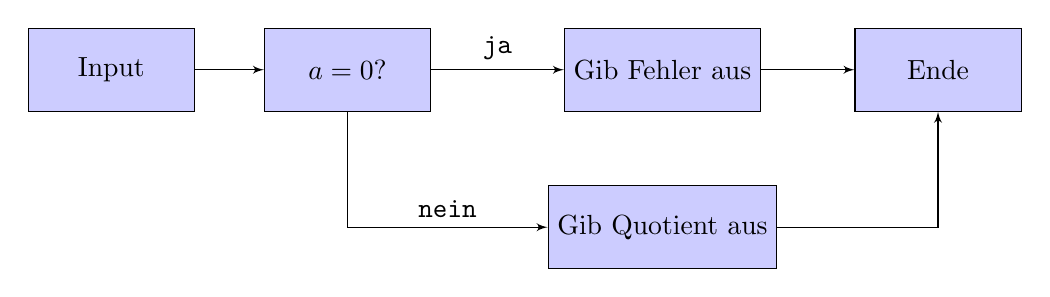
\begin{tikzpicture}[auto, node distance=3cm,>=latex']
        \tikzstyle{block} = [draw, fill=blue!20, rectangle, minimum height=3em, minimum width=6em]

        \node [block] (start) {Input};
        \node [block, right of=start] (if) { $a=0$? };
        \node [block, right of=if, node distance=4cm] (fehler) { Gib Fehler aus };
        \node [block, below of=fehler,node distance =  2cm] (quotient) { Gib Quotient aus };
        \node [block, right of=fehler, node distance = 3.5cm] (ende) { Ende };

        \draw [->] (start) -- node {} (if);
        \draw [->] (if) -- node {\texttt{ja}} (fehler);
        \draw [->] (if.south) |- node [above, near end] {\texttt{nein}} (quotient);
        \draw [->] (quotient) -| node {} (ende);
        \draw [->] (fehler) -- node {} (ende);
    \end{tikzpicture}
\end{center}

Die einfachste Möglichkeit, den Kontrollfluss zu ändern, besteht in so
genannten „bedingten Anweisungen“:
\inputcpp{if.cpp}

In den Zeilen 12 bis 20 sehen wir, wie eine solche Bedingte Anweisung in \Cpp
aussieht. Wir erkennen relativ direkt unser Diagramm hier wieder: In Zeile 12
steht der „$a=0$?“ Block, in den Zeilen 13 bis 17 steht der „Gib Fehler aus“
Block und in Zeile 19 der „Gib den Quotienten aus“ Block.

Beachtet allerding die doppelten Gleichheitszeichen in Zeile 12. \Cpp hat
getrennte Operatoren für Vergleiche und Zuweisungen - Doppelte
Gleichheitszeichen bedeuten Vergleich („sind diese beiden gleich?“), ein
einfaches Gleichheitszeichen bedeutet Zuweisung („mache diese beiden gleich!“).

\textbf{Praxis:}
\begin{enumerate}
    \item Kompiliert \texttt{if.cpp} für den debugger und lasst das Programm im
        gdb laufen. Geht Schritt für Schritt durch das Programm, mit
        verschiedenen Eingaben (wenn ihr am Ende des Programms angekommen seid,
        könnt ihr es mit einem erneuten „run“ neu starten)
    \item Nutzt Google, um herauszufinden, welche anderen Vergleichsoperatoren
        es in \Cpp noch gibt. Versucht, das Programm so zu verändern, dass es
        auf Ungleichheit testet, statt auf Gleichheit (sich sonst aber genauso
        verhält).
    \item Wie würdet ihr testen, ob zwei Zahlen durch einander teilbar sind
        (Tipp: Ihr kennt bereits die Division mit Rest in \Cpp)? Schreibt ein
        Programm, welches zwei Zahlen vom Benutzer entgegen nimmt und ausgibt,
        ob die zweite Zahl die erste teilt.
\end{enumerate}

\textbf{Spiel:}
\begin{enumerate}
    \item Testet mit verschiedenen Eingaben, was passiert, wenn ihr in
        \texttt{if.cpp} statt zwei Gleichheitszeichen nur eines benutzt.
        Benutzt den debugger, um euch den Inhalt von \texttt{b} vor und nach
        dem Test anzuschauen.
    \item Schreibt ein Programm, welches den Benutzer fragt, wie er heißt. Gibt
        der Benutzer euren eigenen Namen ein, soll das Programm begeistert über
        die Namensgleichheit sein, sonst ihn einfach begrüßen.
\end{enumerate}

\lesson{Dateirechte}

Wir machen mal wieder eine kurze Pause von \Cpp um euch ein weiteres wichtiges
Konzept der Linux-Welt nahe zu bringen: Dateirechte.

Unter Windows seid ihr es wahrscheinlich gewohnt, dass der Dateiname festlegt,
wie mit der Datei umgegangen wird -- eine \texttt{.doc} wird in Word geöffnet,
eine \texttt{.zip} in einem installierten Packprogramm, eine \texttt{.bmp}
vermutlich in Windows Paint und eine \texttt{.exe} wird ausgeführt.

Das Konzept der Dateierweiterung hat es auch in die Linuxwelt geschafft, ist
hier aber deutlich weniger wichtig. Insbesondere gibt es keine Dateierweiterung
\texttt{.exe}. Stattdessen hat jede Datei einen bestimmten Modus. Eine Datei
kann ausführbar sein, oder nicht. Sie kann lesbar sein, oder nicht. Sie kann
schreibbar sein, oder nicht. Nicht nur das, jede Datei gehört auch einer
bestimmten Nutzerin und einer bestimmten Nutzerinnengruppe und Ausführbarkeit,
Lesbarkeit oder Schreibbarkeit ist getrennt eingestellt für die Besitzerin der
Datei, der Gruppe, der die Datei gehört und für alle anderen. Eine Datei kann
also z.B. lesbar sein, für alle Nutzerinnen, aber nur eine bestimmte Gruppe von
Nutzerinnen darf sie ausführen und nur eine einzige Nutzerin sie bearbeiten. All
dies wird in neun so gennanten \emph{Permission bits} festgehalten (ein
\emph{Bit} ist die kleinste Einheit an Information, es kodiert genau „ja“ und
„nein“, oder „null“ und „eins“, oder „ein“ und „aus“).

Ihr könnt euch die Besitzerin, die Gruppe, und die permission bits einer Datei
mithilfe von \texttt{ls -l} anschauen. Der output von \texttt{ls -l} ist in
mehreren Spalten angeordnet:
\begin{enumerate}
    \item In der ersten Spalte stehen die Dateiberechtigungen in Form eines 10
        Zeichen langen Strings. Jedes Zeichen steht dabei für ein permission
        bit kann dabei entweder ein \texttt{-}, oder ein Buchstabe sein, wobei
        \texttt{-} bedeutet, dass das entsprechende Bit nicht gesetzt ist. Die
        Bits bedeuten (von links nach rechts gelesen)
        \begin{itemize}
            \item \texttt{\underline{d}irectory}
            \item \texttt{\underline{r}eadable} für die Eigentümerin
            \item \texttt{e\underline{x}ecutable} für die Eigentümerin
            \item \texttt{\underline{w}ritable} für die Eigentümerin
            \item \texttt{\underline{r}eadable} für die Gruppe
            \item \texttt{e\underline{x}ecutable} für die Gruppe
            \item \texttt{\underline{w}ritable} für die Gruppe
            \item \texttt{\underline{r}eadable} für alle Nutzerinnen
            \item \texttt{e\underline{x}ecutable} für alle Nutzerinnen
            \item \texttt{\underline{w}ritable} für alle Nutzerinnen
        \end{itemize}
    \item Nummer an hardlinks (das braucht euch nicht sonderlich interessieren)
    \item Nutzername der Eigentümerin
    \item Gruppe, der die Datei gehört
    \item Dateigröße
    \item Datum der letzten Änderung
    \item Dateiname
\end{enumerate}

Wenn ihr die Berechtigungen von Dateien ändern wollt, könnt ihr dazu
\texttt{chmod} benutzen (wenn ihr wissen wollt, wie man es benutzt: \texttt{man
chmod}), dazu muss sie euch aber gehören. Wenn ihr die Eigentümerin einer Datei
ändern wollt, könnt ihr dazu \texttt{chown} nutzen -- dazu müsst ihr aus
Sicherheitsgründen allerdings Administratorin sein.

\textbf{Praxis:}
\begin{enumerate}
    \item Geht in ein Verzeichnis, in dem eine \texttt{.cpp}-Datei liegt und
        kompiliert sie. Macht ein \texttt{ls -l} und vergleicht die Rechte der
        \texttt{.cpp}-Datei mit der kompilierten Datei.
    \item In der Datei \texttt{/etc/shadow} stehen in verschlüsselter Form
        gespeichert die Kennwörter aller Benutzerinnen auf dem System. Macht ein
        \texttt{ls -l /etc/shadow} und schaut euch die Dateirechte an. Welche
        Bits sind gesetzt?
\end{enumerate}

\textbf{Spiel:}
\begin{enumerate}
    \item Versucht, \texttt{/etc/shadow} in einem Editor zu öffnen.
    \item Legt (z.B. mit dem Texteditor) eine Datei (Es geht nicht um
        Kompilierung, also muss das keine \texttt{.cpp}-Datei sein. Gebt der
        Datei am Besten die Erweiterung \texttt{.txt}) in Eurem Homeverzeichnis
        an und macht sie dann mit \texttt{chmod a+w} world-writable
        (\texttt{a+w} heißt „füge das Recht Schreibbarkeit für alle Nutzerinnen
        hinzu“).  Lasst eure Sitznachbarin die Datei an ihrem Rechner öffnen
        (ihr könnt mittels \texttt{pwd} herausfinden, in welchem Ordner sie
        suchen muss) und euch eine Nachricht hinein schreiben. Schaut nach
        (indem ihr die Datei neu öffnet) ob ihr die Nachricht lesen köntt.
\end{enumerate}

\lesson{Schleifen}

Wir können mit bedingten Anweisungen den Kontrollfluss schon hilfreich
beeinflussen. Aber nicht alle Dinge, die wir unseren Computer anweisen wollen
zu tun, können wir alleine mit bedingten Anweisungen ausdrücken. Wir können
zwar zum Beispiel testen, ob eine Zahl, eine andere teilt. Was aber, wenn wir
testen wollen, ob eine Zahl eine Primzahl ist? Wir könnten jetzt beginnen, jede
Menge bedingter Anweisungen zu machen, „ist die Zahl durch 2 teilbar, wenn ja,
dann ist es keine, sonst teste, ob sie durch 3 teilbar ist, wenn ja, dann ist
es keine, sonst teste, ob sie durch 5 teilbar ist, wenn ja, dann ist es
keine\dots“, aber es sollte offensichtlich sein, dass wir so nur endlich viele
Teilbarkeiten überprüfen können. Wir müssen zwar für jede Zahl nur endlich
viele Teiler überprüfen, aber wenn die Zahl von der Nutzerin eingegeben wird,
wissen wir im Voraus nicht, wie viele das sind!

Für solche Aufgaben wurden Schleifen erfunden. Sie sind ein Mittel, um eine
Menge von Anweisungen häufig auszuführen, solange eine von uns fest gelegte
Bedingung erfüllt ist. Wenn wir zum Beispiel testen wollen, ob eine Zahl eine
Primzahl ist, wäre ein einfacher Algorithmus die so genannte Probedivision:
Gehe von 2 aufwärts alle Zahlen (die kleiner sind, als die Eingabe) durch,
teste, ob sie die Eingabe teilen -- wenn ja, dann handelt es sich nicht um eine
Primzahl. Haben wir alle Zahlen durchprobiert ohne Erfolg, muss es sich um eine
Primzahl handeln.  Wir können das wieder in einem Kontrollflussdiagramm
ausdrücken ($n$ ist dabei die zu testende Zahl, $i$ ist der Teiler, den wir
gerade testen wollen):

\begin{center}
    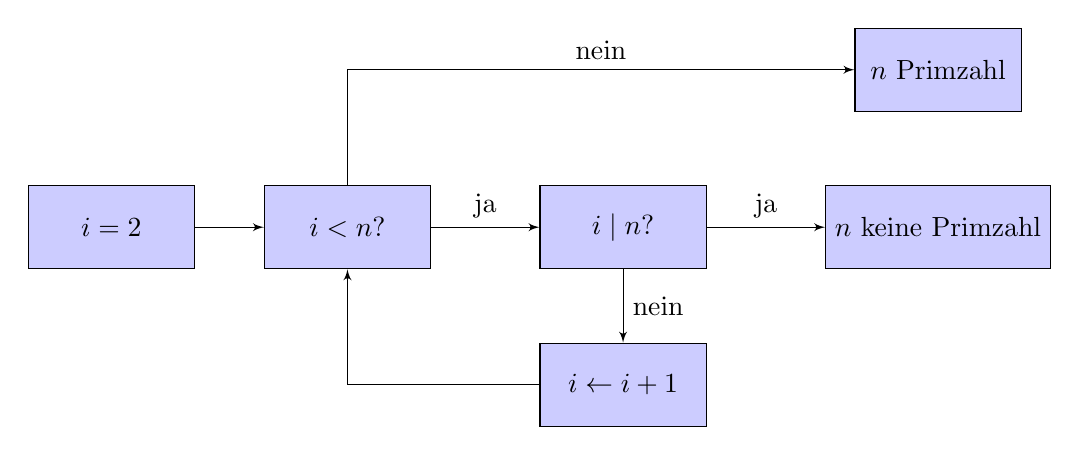
\begin{tikzpicture}[auto, node distance=3cm,>=latex']
        \tikzstyle{block} = [draw, fill=blue!20, rectangle, minimum height=3em, minimum width=6em]

        \node [block] (start) {$i = 2$};
        \node [block, right of=start] (cond) {$i < n$?};
        \node [block, right of=cond, node distance=3.5cm] (if) {$i\mid n$?};
        \node [block, right of=if, node distance=4cm] (nope) {$n$ keine Primzahl};
        \node [block, below of=if, node distance=2cm] (incr) {$i \leftarrow i+1$};
        \node [block, above of=nope, node distance=2cm] (yipp) {$n$ Primzahl};

        \draw [->] (start) -- node {} (cond);
        \draw [->] (cond) -- node {ja} (if);
        \draw [->] (cond) |- node [near end] {nein} (yipp);
        \draw [->] (if) -- node {ja} (nope);
        \draw [->] (if) -- node {nein} (incr);
        \draw [->] (incr) -| node {} (cond);
    \end{tikzpicture}
\end{center}
Das Besondere an Schleifen ist, dass sie geschlossene Kreise zum
Kontrollflussdiagramm hinzufügen. Das erlaubt es uns, die gleiche Anweisung
beliebig oft zu wiederholen.

Wenn wir dieses Kontrollflussdiagramm in \Cpp gießen, sieht dies so aus:
\inputcpp{prim.cpp}

Wie wir sehen, sind Schleifen auch nicht viel schwieriger zu handhaben, als
bedingte Anweisungen. Statt \texttt{if} schreiben wir nun \texttt{while}, sonst
ändert sich am Quellcode nicht viel.

Als kleine Nebenbemerkung sei hier gestattet, dass ihr hiermit nun alle Dinge
kennengelernt habt, um \emph{Turing-vollständig} programmieren zu können, d.h.
ihr könnt alleine mit den Mitteln, die ihr bisher kennen gelernt habt.
\emph{jede} mögliche Berechnung anstellen!

\textbf{Praxis:}
\begin{enumerate}
    \item Versucht, die Arbeitsweise eines debuggers zu simulieren. Geht selbst
        den Quellcode Zeile für Zeile durch, überlegt euch, was die Zeile tut
        und welchen Inhalt die Variablen haben. Überlegt euch dann, wohin der
        Computer (bei Kontrollflussstrukturen) als nächstes springen würde.
        Wenn ihr nicht weiter wisst, kompiliert das Programm für den debugger,
        startet es im debugger und geht es durch.
    \item Warum funktioniert das Programm für den Fall $n = 2$?
    \item Schreibt selbst ein Programm, welches eine Zahl von der Nutzerin
        entgegennimmt und dann bis zu dieser Zahl hochzählt.
    \item Modifiziert euer Programm, sodass es von dieser Zahl bis zu 0
        hinunterzählt.
\end{enumerate}

\textbf{Spiel:}
\begin{enumerate}
    \item Das Programm funktioniert noch nicht korrekt, wenn man 1 eingibt
        (denn 1 ist keine Primzahl). Modifiziert es, sodass es auch für 1
        funktioniert.
    \item Kompiliert \texttt{whiletrue.cpp} und führt es aus. Was beobachtet
        ihr? Warum? (Ihr könnt das Programm abbrechen, indem ihr
        \texttt{Strg+C} drückt)
\end{enumerate}

\inputcpp{whiletrue.cpp}

\lesson{Coding style}

Wir haben mitlerweile hinreichend viele verschiedene Verschachtelungen im
Quellcode kennen gelernt, dass es sich lohnt, ein paar Worte über coding styĺe
zu sprechen.

Schon wenn ihr euch während dieses Kurses an einen von uns wendet und um Hilfe
bittet, ergibt sich das Problem der Lesbarkeit von Quellcode. Um euch zu
helfen, sollte man möglichst mit einem Blick erfassen können, was euer Code
tut, wie er strukturiert ist, welche Variable was bedeutet. Um dies zu
unterstützen, gibt es mehrere Dinge, auf die man achten kann.

\begin{description}
    \item[Einrückung]
        Wie euch vermutlich aufgefallen ist, sind an verschiedenen Stellen im
        Code einzelne Zeilen ein wenig eingerückt. Dies ist vermutlich das
        wichtigste Werkzeug, welches zur Verfügung steht, um die Lesbarkeit von
        Code zu unterstützen (auch, wenn es nicht nötig ist, um formal korrekte
        Programme zu schreiben). Die einzelnen Einheiten des Kontrollflusss
        werden dadurch visuell voneinander abgegrenzt, was es einfacher macht,
        den Programmverlauf zu verfolgen.

        Wie genau eingerückt werden sollte, darüber scheiden sich die Geister.
        Man kann mit mehreren Leerzeichen oder durch Tabulatoren einrücken.
        Empfehlenswert ist auf jeden Fall, mehrere gleichförmige „Ebenen“ zu
        haben (z.B. 4,8,12,\dots Leerzeichen zu Beginn der Zeile). Eine
        Faustregel für gut lesbare Einrückung ist, immer wenn man eine
        geschweifte Klammer öffnet, eine Ebene tiefer einzurücken und immer,
        wenn man eine geschweifte Klammer schließt, wieder eine Ebene zurück zu
        nehmen.
    \item[Klammern]
        Aus der Schule kennt ihr das Prinzip „Punkt- vor Strichrechnung“. Dies
        ist eine Regel, die so genannte \emph{Präzedenz} ausdrückt, also die
        Reihenfolge, in der Operatoren ausgewertet werden. Punkt vor Strich ist
        allerdings nicht aussreichend, um vollständig zu beschreiben, wie sich
        Operatoren in Gruppen verhalten. Schaut euch z.B. den Ausdruck
        \texttt{2 * 3 / 2} an. Da der Computer Ganzzahldivision benutzt, kommen
        hier unterschiedliche Ergebniss raus, je nachdem, ob zunächst das
        \texttt{*} oder das \texttt{/} ausgewertet wird. Im ersten Fall
        erhalten wir \texttt{6 / 2 == 3}, wie wir erwarten würden. Im zweiten
        Fall wird aber abgerundet, sodass wir \texttt{2 * 0 == 0} erhalten.

        Um solche und ähnliche Uneindeutigkeiten zu vermeiden, bietet es sich
        an, Klammerung zu verwenden. Selbst wenn wir im obigen Fall
        \emph{wissen} in welcher Reihenfolge die Operatoren ausgewertet werden,
        jemand der unseren Code liest weiß das vielleicht nicht. Einfach von
        vornherein die gewollte Reihenfolge der Auswertung zu klammern
        verhindert Verwirrung bei uns über das Verhalten des Computers, als
        auch bei Menschen, die später wissen wollen, was wir meinten.
    \item[Kommentare]
        Wir haben schon in mehreren Quellcodedateien Kommentare verwendet, um
        einzelne Dinge zu erklären. Insgesamt bietet es sich an, dies selbst
        ebenfalls zu tun, um den Programmfluss dem Leser von Quellcode klar zu
        machen. Das heißt nicht, dass man jede Anweisung noch einmal mit einem
        Kommantar versehen sollte, der sie ausführlich erklärt, aber an
        wichtigen Punkten können einem kurze Kommentare das Leben enorm
        vereinfachen. Und ihr dürft nicht vergessen, dass ihr euch vielleicht
        selbst in ein oder zwei Jahren noch einmal euren eigenen Quellcode
        anschauen müsst und ihr werdet wirklich überrascht sein, wie wenig ihr
        von dem Zeug, welches ihr selbst geschrieben habt verstehen werdet.
    \item[Leerzeichen]
        Weniger wichtig als die ersten drei Punkte können trotzdem gezielte
        Leerzeichen (z.B. zwischen Operatoren und Operanden in arithmetischen
        Ausdrücken) die Lesbarkeit enorm erhöhen. Gerade in arithmetischen
        Ausdrücken ist es eine gute Angewohnheit.
\end{description}

Es gibt sicher noch viele Regeln, über die ihr im Laufe eures Lebens stolpern
werdet, wenn ihr euch entschließen solltet, regelmäßig zu programmieren. Häufig
werdet ihr euch darüber ärgern, manchmal zu recht. Aber versucht im Zweifel
einen halbwegs sauberen Stil auch als euren eigenen Verbündeten zu sehen, denn
ob es nun vergessene Klammern, Semikolons oder versteckte Fehler in der
Operatorpräzedenz sind, ein sauberer Stil kann euch bei allen enorm helfen, sie
aufzuspüren.

\textbf{Praxis:}
\begin{enumerate}
    \item Eine weit verbreitete einfache Aufgabe, die in Bewerbungsgesprächen
        auf Stellen als Programmiererin häufig gestellt wird, ist
        \emph{FizzBuzz}. In \texttt{fizzbuzz.cpp} ist eine möglich Lösung für
        diese Aufgabe gegeben. Könnt ih r (nur mittels des Quellcodes) sagen,
        was das Programm tut?
    \item Nutzt die oben gegebenen Faustregeln, um den Quellcode lesbarer zu
        machen. Ihr müsst nicht alles bis aufs Wort befolgen, macht einfach so
        lange weiter, bis ihr findet, man kann hinreichend schnell verstehen,
        was hier passieren soll.
\end{enumerate}

\inputcpp{fizzbuzz.cpp}

\textbf{Spiel:}
\begin{enumerate}
    \item Entfernt in eurem veränderten Quellcode eine geschweifte Klammer
        eurer Wahl. Lasst eure Sitznachbarin über den Quellcode schauen und die
        fehlende Klammer finden.
\end{enumerate}

\lesson{Funktionen}

Aus der Mathematik kennt ihr bereits Funktionen, wie zum Beispiel $f(x) = 4x^3 - 8x^2 + 16x - 12$.
Eine wichtige Idee dahinter ist es einfach $f(3)$ zu schreiben, wenn man eigentlich $4 \cdot 3^3 - 8 \cdot 3^2 + 16 \cdot 3 - 12$ meint.
Da dies häufig vorteilhaft ist, wurde diese Funktionalität in die meisten Programmiersprachen übernommen.

Eine Funktion in \Cpp besteht aus zwei Teilen: der \emph{Signatur} und dem \emph{Funktionsrumpf}.
Die Kombination von Parametertypen und Rückgabetyp bildet die Signatur einer Funktion.
Parameter sind Werte, die der Funktion übergeben werden, zum Beispiel das $x$ in $f(x)$.
Für eine Funktion \cppinline{my_func}, die  $x^n$ berechnen soll, könnte eine Signatur so aussehen:

\begin{center}
	\cppinline{double my_func(double x, int n)}
\end{center}

%Signatur Diagramm von Koebi? Ich kriege nichts schönes hin

Diese Signatur besteht also aus einem Datentypen, der den Rückgabetypen der Funktion bestimmt, direkt gefolgt von dem Namen der Funktion, der beliebig gewählt werden kann.
Und dahinter in Klammern werden die einzelnen Paramter durch Komma getrennt angeben, wobei ein Paramter immer aus dem Datentyp des Paramters und einem beliebigen Namen für den Paramter besteht.
In diesem Fall ist also \texttt{double} der Rückgabewert, \cppinline{my_func} der Name, \cppinline{x} ein Parameter mit dem Typ \texttt{double} und \cppinline{n} ein Paramter mit dem Typ \texttt{int}.
Damit können dann Werte an die Funktion in der Form \cppinline{my_func(1.41, 2)} übergeben werden.

An dieser Stelle ist der Unterschied zwischen Rückgabe und Ausgabe wichtig: Eine Ausgabe (gekennzeichnet durch \cppinline{std::cout}) gibt Informationen auf dem Bildschirm für die Nutzerin aus, eine Rückgabe (gekennzeichnet durch \texttt{return}) gibt hingegen ein bestimmtes Ergebnis an einen anderen Teil des Programmes zurück, damit dieser dort in einer Variable gespeichert oder direkt weiter verarbeitet werden kann.
Dabei kann man sich vorstellen, dass der Funktionsaufruf nach dem die Funktion ausgeführt wurde durch den Rückgabewert ersetzt wird.
Dies könnte für die Funktion \cppinline{my_func} folendermaßen aussehen:

\begin{center}
	\cppinline{f(5.0 + f(3.0, 2), 3)} $\mapsto$ \cppinline{f(5.0 + 9.0, 3)} $\mapsto$ \cppinline{f(14.0, 3)} $\mapsto$ \cppinline{2744}
\end{center}


Der Funktionsrumpf beinhaltet den Code, der beim Funktionsaufruf tatsächlich ausgeführt wird.
Dieser wird wie in einer Schleife von \mintinline{c++}|{| und \mintinline{c++}|}| umschlossen.
Innerhalb dieser Klammern kann dann beliebiger Code ausgeführt werden, wie auch in der \texttt{main}-Funktion.
Dabei kann auf die Parameter einfach mit dem in der Signatur definierten Namen zugegriffen werden.
Also in unserem Beispiel mit \cppinline{x} und \cppinline{n}.
Vor dem Ende des Funktionsrumpfes muss eine Rückgabe mit \texttt{return} ausgeführt werden.
Das kann zum Beispiel so \texttt{return x;} oder so \texttt{return 5;} aussehen.

Funktionen werden beispielsweise benötigt, wenn bestimmte Programmteile häufiger mit verschiedenen Parametern ausgeführt werden sollen.
Die Collatz-Vermutung\footnote{\url{https://de.wikipedia.org/wiki/Collatz-Vermutung}} besagt für die Folge:
\[
	x_n =
	\begin{cases}
		\frac{x_{n-1}}{2} & x_{n-1} \text{ ist gerade} \\
		3 \cdot x_{n-1} + 1 & x_{n-1} \text{ ist ungerade}
	\end{cases}
\]
dass jeder Startwert $x_1$ aus den natürlichen Zahlen nach endlich vielen Schritten bei der $1$ angelangt.
Zum Beispiel für den Startwert $x_1 = 42$:

\[
    42 \mapsto 21 \mapsto 64 \mapsto 32 \mapsto 16 \mapsto 8 \mapsto 4 \mapsto 2 \mapsto 1 \mapsto 4 \mapsto 2 \mapsto 1 \mapsto \ldots
\]

Wenn nun die Frage aufkommt was die nächsten Folgenglieder von verschiedenen Zahlen sind, wäre ein möglicher Lösungsweg eine Funktion zu schreiben, die der Nutzerin die nächste Zahl in dieser Folge zurückgibt.

\inputcpp{funktion.cpp}

\textbf{Praxis:}
\begin{enumerate}
	\item Verändert das Programm in \texttt{funktion.cpp} so, dass es nicht die einzelnen Zahlen \texttt{x1}, \texttt{x2} und \texttt{x3}, sondern die Summe dieser ausgibt.
%Wirkt wie Kinderkram nicht zum Funktionskapitel, möchte aber nochmal den Unterschied zwischen Ausgabe und Rückgabe dadurch nochmal klarer machen
	\item Kompiliert das angepasste Programm und lasst es im debugger Schritt für Schritt durchlaufen, setzt dafür wieder einen breakpoint für die \texttt{main}-Funktion.
	    Sobald der debugger euch anzeigt, als nächstes die Funktion ausführen zu wollen, \texttt{step} statt \texttt{next} aufrufen, sodass der debugger in die Funktion hineinspringt.
	\item Schreibt eine Funktion (nach der Funktion \texttt{collatz} und vor \texttt{main}), die einen \texttt{int} entgegen nimmt und die Anzahl der Schritte bestimmt bis die Folge bei der 1 angekommen ist und diese als \texttt{int} zurückgibt.
	    Benutzt dafür die bereits vorhandene Funktion \texttt{collatz}.
	\item Schreibt euer Programm so um, dass es eine Zahl von der Nutzerin entgegen nimmt und die Anzahl der Schritte ausgibt, bis diese Zahl zu einer 1 wird.
\end{enumerate}

\textbf{Spiel:}
\begin{enumerate}
    \item Was passiert, wenn ihr in einer Funktion den \texttt{return}-Ausdruck vor dem Ende eurer Funktion benutzt?
    \item Vertauscht in \texttt{funktion.cpp} die Funktion \texttt{collatz} mit der Funktion \texttt{main} (verschiebt also die gesamte Funktion \texttt{collatz} an das Ende der Datei).
        Versucht, die Datei zu kompilieren.
        Was ist die Fehlermeldung des Compilers?
    \item Verschiebt die Funktion \texttt{collatz} \emph{in} die \texttt{main}-Funktion (also irgendwo nach der öffnenden geschweiften Klammern, aber vor die dazu gehörige schließende).
        Versucht, die Datei zu kompilieren. Was ist die Fehlermeldung des Compilers?
    \item Implementiert die Funktion, die $x^n$ umsetzt, ignoriert dabei zunächst negative Exponenten. \\
        (\emph{Tipp:} Die Signatur ist bereits oben gegeben, für den Funktionsrumpf könnten sich Schleifen eignen.)
    \item Ihr könnt eure Funktion von innerhalb wieder aufrufen. Versucht eure Funktion auf negative Exponenten zu erweitern, indem ihr benutzt, dass gilt $x^{-n} = \frac{1.0}{x^n}$.
    \item Schaut euch eure bisherigen Lösungen an.
        Findet ihr noch häufiger Stellen, an denen ihr einzelne Teilprogramme in Funktionen auslagern könnt?
\end{enumerate}

\lesson{Die \Cpp Standardbibliothek}

Vielleicht habt ihr euch irgendwann gewundert, was eigentlich das
\texttt{std::} ist, was wir vor so viele Dinge schreiben. Warum müssen wir es
z.B. vor \texttt{string} schreiben, aber nicht vor \texttt{int}?

Die Antwort auf die Frage ist die \Cpp Standardbibliothek. So wie eigentlich
jede Programmiersprache, definiert sich \Cpp nicht nur durch die \emph{Syntax}
-- also die genaue Spezifikation, wie ein Quellcodeprogramm aufgebaut ist, wie
eine Anweisung aussieht und ob wir z.B. ein Semikolon am Ende jeder Anweisung
brauchen -- sondern auch über die im Sprachumfang enthaltene
Standardbibliothek, die einem nützliche Funktionen und Objekte für Ein- und
Ausgabe, komplexe Datentypen oder zur Interaktion mit dem Betriebssystem gibt.

\Cpp nutzt das Prinzip von so genannten \emph{Namespaces}. Das ist eine
Möglichkeit, eine Gruppe von Datentypen, Funktionen und Variablen unter einem
gemeinsamen Namen zu verpacken. Stellt euch vor, ihr wollt in eurem Programm
eine Funktion \texttt{random} definieren. Ihr hättet ganz schön große Problem,
denn der Compiler wüsste dann, wenn ihr \texttt{random} schreibt nicht, ob ihr
eure eigene Funktion meint, oder ob ihr die Standard-\Cpp Funktion meint.

Aus diesem Grund leben alle Funktionen und Objekte der \Cpp Standardbibliothek
im Namespace \texttt{std}. Um auf sie zuzugreifen, müsst ihr dem Compiler
sagen, aus welchen Namespace ihr sie haben wollt, dazu schreibt ihr eben den
Namen des Namespaces und zwei Doppenpunkte vor den Namen der Variablen (oder
Funktion), also ist \texttt{std::cout} „Die Variable \texttt{cout} aus dem
Namespace \texttt{std}“.

\inputcpp{namespaces.cpp}

\textbf{Praxis:}
\begin{enumerate}
    \item Was gibt dieses Programm aus, wenn man es kompiliert und ausführt?
        Überlegt es euch zuerst selbst, dann probiert es aus.
\end{enumerate}

Wenn ihr wissen wollt, was die Standardbibliothek alles so für euch bereit
stellt, könnt ihr euch in der Referenz der Standardbibliothek unter

\url{http://www.cplusplus.com/reference/}

umschauen. Es ist nicht ganz einfach, zu wissen, wo man dort findet, was man
sucht, in dem Fall kann Google ein im Regelfall ganz gut helfen. Wenn man
einmal weiß, \emph{was} man sucht, findet man in der Referenz vor allem,
\emph{wie} man es benutzt.

Die Standardbibliothek ist aufgeteilt auf so genannt \emph{Headerdateien}, die
wir mittels \texttt{\#include} benutzen können. Diese Header sind, worunter ihr
zuerst wählt, wenn ihr auf obige url geht. Jeder Header definiert dann eine
Menge an Funktionen, Typen und Klassen (was genau eine Klasse ist, lernt ihr
spätestens in der Vorlesung).

\textbf{Praxis:}
\begin{enumerate}
    \item Findet in der \Cpp-Referenz eine Funktion, um die aktuelle Zeit
        auszugeben. Schreibt ein Programm, welches die Aktuelle Zeit ausgibt
        (es reicht, einen so genannten \emph{Unix timestamp} auszugeben). Ihr
        könnt die Ausgabe eures Programms mit der Ausgabe von \texttt{date
        +\%s} vergleichen, um es zu testen.
    \item Mit der Funktion \texttt{rand()} könnt ihr Zufallszahlen generieren
        (ihr braucht dazu den Header \texttt{<cstdlib>}). Schreibt ein
        Programm, welches vom Benutzer eine Zahl entgegennimmt und diese Anzahl
        Zufallszahlen ausgibt. Führt das Programm mehrfach aus. Was fällt auf?
    \item Konsultiert die \Cpp-Referenz, um heraus zu finden, wo das Problem
        liegt. Könnt ihr es beheben?
\end{enumerate}

\lesson{Arrays}

Als nächstes wichtiges Konzept in \Cpp werden wir uns \emph{Arrays} anschauen.
Arrays sind eine Möglichkeit, mehrere Elemente des gleichen Typs zusammen zu
fassen. Statt also einer Stelle im Speicher, an der ein \texttt{int} liegt,
habt ihr einen ganzen Speicherbereich, in dem 100 (oder eine beliebige andere
Anzahl an) \texttt{int}s liegen.

Die Elemente in einem Array sind durchnummeriert, man nennt die Nummer eines
Arrayelements seinen \emph{Index}. Das erste Element hat den Index 0, das
zweite den Index 1 und das 100te hat den Index 99 -- Vorsicht also, der höchste
Index in einem Array mit 100 Elementen ist 99, nicht 100! Um ein Array zu
definieren, schreibt ihr hinter seinen Namen eine eckige Klammer auf, die
Anzahl an Elementen, die es enthalten soll, und eine eckige Klammer zu. Auf ein
bestimmtes Arrayelement zuzugreifen könnt ihr tun, indem ihr seinen Index in
eckigen Klammern hinter den Namen schreibt. Folgendes Programm macht
hoffentlich die Syntax klar:
\inputcpp{array.cpp}

Es gibt einige Dinge, zu beachnten, wenn ihr mit Arrays arbeitet. Das
wichtigste ist oben schon genannt -- sich davon verwirren zu lassen, dass
Indizes bei 0 anfangen und aus Versehen über das Array hinaus schreiben oder
lesen ist ein so häufiger Fehler, dass er seinen eigenen Namen bekommen hat:
„Off-by-one error“. Wichtig ist, dass der Compiler diesen Zugriff nicht
verhindern wird! Das ist von daher eine sehr fiese Sache, als dass dieser
Fehler auch beim Ausführen nicht immer Probleme machen wird -- aber manchmal
lässt er auch euer Programm spontan abstürzen in einem so genannten
\emph{segmentation fault}.

Eine Limitation von Arrays, die ihr beachten solltet, ist, dass bereits zur
Compilezeit fest stehen muss, wie viele Elemente sie enthalten sollen. Ihr
könnt also z.B. nicht die Nutzerin fragen, wie viele Elemente in das Array
passen soll, denn dies würde erst zur Laufzeit feststehen (wir werden später
noch Wege um diese Limitation kennen lernen).

Ihr könnt auch Arrays von Arrays (so genannte zweidimensionale Arrays)
erstellen, indem ihr zweimal in eckigen Klammern die Größe des Arrays
hinschreibt. Die erste Größe gibt dann die Anzahl der Zeilen an, die zweite die
Anzahl der Spalten. Auch beim Zugriff auf Arrayelemente müsst ihr dann zwei
Indizes angeben. Wir werden dies später noch nutzen, hier sei erst einmal nur
die generelle Möglichkeit genannt.

\textbf{Praxis:}
Wir wollen die Seite \url{http://www.ich-kann-mich-nicht-entscheiden.de/}
nachmachen und eine Entscheidungshilfe programmieren, die aus mehreren von der
Nutzerin gegebenen Möglichkeiten eine per Zufall auswählt.

\begin{enumerate}
    \item Schreibt zunächst ein Programm, welches ein Array aus 10 Strings
        erstellt und die Nutzerin 10 mal nach einer Antwortmöglichkeit fragt
        und die gegebenen Antworten nacheinander in das Array schreibt.
    \item Fügt nun die Möglichkeit zu, weniger Antworten anzugeben. Dazu könnt
        ihr zum Beispiel zuerst fragen, wie viele Antwortmöglichkeiten es geben
        soll und dann so oft fragen (und natürlich einen Fehler ausgeben, wenn
        es mehr als 10 Antworten geben soll).
    \item Ihr könnt dann (so wie in dem Programm oben) eine Zufallszahl
        erzeugen. Um sicher zu gehen, dass sie nicht zu groß wird, könnt ihr
        den Rest bei Teilung durch Anzahl der eingegebenen Antworten nehmen
        (sind z.B. 7 Antworten angegeben und die Zufallszahl ist 25778, so wäre
        der resultierende Index \texttt{25778 \% 7 == 4}). Gebt dann die
        Antwortmöglichkeit aus, die dem zufallsgeneriertem Index
        entspricht.
\end{enumerate}

Sollte euer Programm einmal nicht korrekt kompilieren, denkt daran die
Fehlermeldung sorgfältig zu lesen, damit sie euch Aufschluss über die
Fehlerursache gibt. Sollte euer Programm zwar kompilieren, sich dann aber
komisch verhalten, denkt daran, den debugger zu benutzen und es Schritt für
Schritt durchzugehen, um die Fehlerquelle zu finden. Solltet ihr trotz alledem
nicht weiter kommen, oder nicht wissen, was von euch erwartet wird, fragt einen
von uns.

\textbf{Spiel:}
\begin{enumerate}
    \item Schreibt ein Progamm, welches ein Array beliebiger Größe erstellt und
        dann auf einen Index weit ausserhalb des erlaubten Bereichs schreibt.
        Was beobachtet ihr?
    \item Implementiert das \emph{Sieb des Eratosthenes}
        \footnote{\url{https://de.wikipedia.org/wiki/Sieb_des_Eratosthenes}},
        wenn ihr noch nicht ausgelastet seid.
        Denkt daran, es initial zu befüllen und denkt euch eine clevere
        Möglichkeit auf, das „Streichen“ zu realisieren.
\end{enumerate}

\lesson{Warnings}

Wir haben uns bereits ausführlich mit den Fehlermeldungen des Compilers
auseinander gesetzt. Wir haben auch festgestellt, dass es viele Fehler gibt,
die uns der Compiler durchgehen lässt, die aber im späteren Programmlauf zu
Problemem führen können. Und wir haben den debugger kennengelernt, um die
Ursache solcher Fehler zu finden und sie beheben zu können. Nun wollen wir uns
anschauen, wie wir den Compiler in gewisser Weise „wachsam“ machen können,
sodass er uns auch über Dinge informiert, die zwar keine Fehler sind, aber
möglicherweise zu unerwartetem Verhalten führen können.

\textbf{Praxis:}
\begin{enumerate}
    \item Kompiliert \texttt{warnings.cpp}. Testet das Program mit
        verschiedenen Eingaben. Was beobachtet ihr?
\end{enumerate}
\inputcpp{warnings.cpp}

Fehler wie diese können nicht mehr auftreten, wenn ihr \emph{warnings}
anschaltet. Dies passiert über weiter Optionen, die wir dem Compiler mitgeben.

\textbf{Praxis:}
\begin{enumerate}[resume]
    \item Kompiliert \texttt{warnings.cpp} mittels \texttt{g++ -Wall -o
        warnings warnings.cpp}.
\end{enumerate}

Warnings sehen im Wesentlichen genauso aus, wie Fehler. Der einzige Unterschied
ist, dass statt \texttt{error} in der Zeile ein \texttt{warning} steht und dass
der Compiler zwar die Meldung ausgibt, aber trotzdem ganz normal das Programm
erzeugt. Trotzdem solltet ihr warnings ernst nehmen. Die meisten „ernsthaften“
Programmierer aktivieren warnings, da die meisten davon gefundenen Meldungen
tatsächlich behoben werden sollten.

Ihr könnt mit verschiedenen Parametern beeinflussen, welche warnings euch der
Compiler anzeigt und wie er damit umgeht. Wir wollen hier nur drei nennen:

\begin{description}
    \item[-Wall]
        Aktiviert „alle“ warnings. Tatsächlich stimmt das so nicht, aber wenn
        ihr immer daran denkt, diesen Parameter anzugeben, solltet ihr bereits
        den allergrößten Teil der vom Compiler entdeckbaren Probleme, die ihr
        erzeugt, abfangen können.
    \item[-Wextra]
        Aktiviert noch ein paar warnings (ihr seht, warum „alle“ in
        Anführungszeichen stand). In einigen Fällen sind auch die hier
        aktivierten warnings für euch relevant.
    \item[-Werror]
        Dieser Parameter führt dazu, dass jede warning als Fehler behandelt
        wird, d.h. der Compiler bricht ab, wenn er eine warning produzieren
        würde. Dieser Parameter ist hochumstritten und in der Praxis sollte man
        ihn eigentlich nicht einsetzen. Für Beginner kann er aber hilfreich
        sein, da er von vornherein antrainiert, warnings ernst zu nehmen und
        sie nicht einfach zu ignorieren.
\end{description}

Wenn ihr bei jedem Compilerlauf nun warnings anschalten wollt -- und am Besten auch noch für den debugger, falls ihr ihn braucht -- wird der Befehl zum Kompilieren langsam sehr lang. Für die Dauer des Vorkurses könnt ihr euch mittels

\texttt{alias\footnote{alias ist ein shell-befehl, der euch eine Reihe von
Anweisungen und Befehlen neu benennen lässt. In diesem Fall ist danach zum
Beispiel der noch nicht existente Befehl \texttt{compile} ein neuer Name für
\texttt{g++ -Vall -Wextra -Werror -O0 -g3}. Beachtet, dass ihr hier genau das
abtippen müsst, was da steht, mit Leerzeichen und allem} compile="g++ -Wall
-Wextra -Werror -O0 -g3"}

ein bisschen Arbeit ersparen. Ein einfaches \texttt{compile -o foo foo.cpp}
wird dann automatisch den Compiler mit allen angegebenen Optionen aufrufen. Den
\texttt{alias} müsst ihr allerdings jedes mal, wenn ihr in der Zwischenzeit ein
Terminal geschlossen habt, neu ausführen, denn er geht bei Schließung eines
Terminals verloren!

\textbf{Praxis:}
\begin{enumerate}[resume]
    \item Mit der warning in \texttt{warnings.cpp} möchte euch der Compiler
        darauf hinweisen, dass ihr hier eine Zuweisung macht, obwohl ein
        Wahrheitswert erwartet wird. Es gibt zwei Möglichkeiten, die warning zu
        beheben: Ihr könnt Klammern um die Zuweisung machen (und dem Compiler
        so sagen, dass ihr euch sicher seid, dass hier eine Zuweisung hinsoll),
        oder ihr könnt aus der Zuweisung einen Vergleich machen. Welche
        Möglichkeit erscheint euch angebracht? Setzt sie um und kompiliert das
        Programm erneut (mit warnings).
    \item In \texttt{warnprim.cpp} haben wir einen Fehler eingebaut. Kompiliert
        das Programm mit warnings und korrigiert ihn.
\end{enumerate}

\inputcpp{warnprim.cpp}

\textbf{Spiel:}
\begin{enumerate}
    \item Die Auswirkungen von warning-Parametern hängen stark von anderen
        Parametern ab. Wir benutzen z.B. häufiger einmal den Parameter
        \texttt{-O0}. Dieser legt das Level an \emph{Optimierung} fest, also
        wie sehr euer Compiler versucht, euren Code umzustrukturieren, sodass
        er sich gleich verhält, aber schneller läuft. \texttt{-O2} würde
        bedeuten, dass relativ stark optimiert wird.

        \texttt{zaehlen.cpp} enthält ein Programm, um bei einem von der Nutzerin eingegebenen Wort zu zählen, wie oft ein bestimmter Buchstabe (zurzeit \texttt{a} vorkommt).
        Kompiliert es mit \texttt{g++ -Wall -O2 -o zaehlen zaehlen.cpp} (probiert es auch einmal ohne \texttt{-O2} oder ohne \texttt{-Wall}) und schaut euch die resultierende Warning an.
        Benutzt gegebenenfalls Google, um heraus zu finden, was sie bedeutet und wie ihr sie beheben könnt.
\end{enumerate}

\inputcpp{zaehlen.cpp}

\lesson{Tic Tac Toe - Teil 1}

Nachdem wir jetzt lange dröge und unspannende -- und zum Teil einfach
un\emph{sinnige} -- Lektionen und Beispiele hatten, wollen wir uns als Ende von
Kapitel 1 einer ein wenig spannenderen Aufgabe widmen -- wir wollen ein
einfaches Spiel programmieren. Wir haben dazu Tic Tac Toe ausgewählt, da es
relativ überschaubare Spiellogik besitzt. Ein- und Ausgabe, werden wir über die
Konsole machen.

In \texttt{vorkurs/lektion17} findet ihr eine Datei \texttt{tictactoe.o}. Diese
könnt ihr nicht in eurem Editor öffnen - sie enthält von uns bereitgestellte,
bereits vorkompilierte Funktionen, die ihr nutzen könnt, um einen Anfang zu
haben. Wir werden sie später Stück für Stück ersetzen.

Um die Funktionen zu nutzen, müsst ihr zwei Dinge tun: Ihr müsst sie einerseits
in eurem Sourcecode \emph{deklarieren}, andererseits müsst ihr sie beim
Kompilieren mit \emph{linken}.

Die Deklaration erfolgt ganz ähnlich, wie ihr auch vorgehen würdet, wenn ihr
die Funktion selbst schreiben würdet: Ihr schreibt Rückgabetyp, Namen und
Parameter der Funktion auf. Statt des Funktionenkörpers in geschweiften
Klammern, beendet ihr die Zeile mit einem Semikolon. Da wir die Funktion aus
einer anderen Datei laden wollen, müssen wir noch ein \texttt{extern}
voranstellen. In \texttt{tictactoe.cpp} ist dies am Beispiel von
\texttt{frage\_feld\_nummer} vorgemacht.

\texttt{tictactoe.o} definiert euch insgesamt folgende Funktionen:
\begin{description}
    \item[frage\_feld\_nummer]
        Nimmt ein Array von \texttt{int}s der Länge 9 entgegen und gibt einen
        \texttt{int} zurück.

        Gibt auf der Konsole eine Frage nach der Feldnummer aus
        (durchnummeriert von 0 bis 8), liest eine Feldnummer von der Nutzerin
        ein und gibt diese zurück. Die Funktion stellt sicher, dass die
        Feldnummer zwischen 0 und 8 liegt und dass das Feld noch nicht besetzt
        ist (sonst wird noch einmal nachgefragt).
    \item[gebe\_feld\_aus]
        Nimmt ein Array von \texttt{int}s der Länge 9 entgegen und hat als
        Rückgabetyp \texttt{void} (was für „keine Rückgabe“ steht).

        Gibt das gegebene Feld auf der Konsole aus. Dabei werden die 9 Felder
        von oben links nach unten rechts von 0 beginnend durchnummeriert. Das
        9-elementige Array stellt also das Feld dar. Eine 0 in einem
        Arrayelement bedeutet, dass das Feld leer ist, eine 1 bedeutet, dass
        sich dort ein Kreuz befindet und eine 2 bedeutet, dass sich ein O dort
        befindet. Andere Werte werden mit einem \texttt{?} dargestellt.
    \item[gewinnerin]
        Nimmt ein Array von \texttt{int}s der Länge 9 entgegen und hat als
        Rückgabetyp \texttt{int}.

        Prüft, ob in diesem Zustand des Feldes bereits eine der Spielerinnen
        gewonnen hat. Die Funktion gibt 0 zurück, wenn noch niemand gewonnen
        hat, 1, wenn die Spielerin X gewonnen hat und 2, wenn die Spielerin O
        gewonnen hat. Sollte das Spiel unentschieden ausgegangen sein, wird
        eine 3 zurück gegeben.
\end{description}

Der zweite Teil, den ihr zur Benutzung der Funktionen braucht ist das Linken
(was genau das bedeutet, wird später noch erklärt). Dies ist fürs Erste sehr
einfach: Ihr gebt einfach dem \texttt{g++} Befehl zusätzlich zu eurer
\texttt{.cpp} Datei noch \texttt{tictactoe.o} als zusätzliche Inputdatei an.

\inputcpp{tictactoe.cpp}

\textbf{Praxis:}
\begin{enumerate}
    \item Ergänzt \texttt{tictactoe.cpp} um Deklarationen für die anderen
        beschriebenen Funktionen aus \texttt{tictactoe.o}. Ein Array als
        Parameter könnt ihr in genau der gleichen Notation angeben, wie ihr es
        euch in einer Funktion als Variable definieren würdet.
    \item Das Grundgerüst eines Spiels ist die \emph{input-update-display}-loop.
        Dies ist eine Endlosschleife, in der zunächst der \emph{input} der
        Spielerin abgefragt wird. Anschließend wird der interne Spielzustand
        aktualisiert (\emph{update}). Zuletzt wird der neue Spielzustand
        angezeigt (\emph{display}). Der anfängliche Spielzustand wird vor
        dieser loop hergestellt (\emph{setup}).

        \texttt{tictactoe.cpp} zeigt dieses Grundgerüst. Ergänzt den input- und
        den display-Teil mithilfe der gegebenen Funktionen. Ergänzt auch den
        setup-Teil; ihr braucht für den Spielzustand einerseits das Array,
        welches das Spielfeld fassen soll, andererseits eine Variable für die
        Spielerin, die gerade am Zug ist und eine Variable, die das im
        aktuellen Zug eingegebene Feld speichert.
    \item Nun müssen wir noch den Update-Teil ergänzen. Hier solltet ihr in das
        von der aktuellen Spielerin gewählte Feld mit deren Nummer füllen,
        testen, ob jemand gewonnen hat und wenn ja, die Siegerin ausgeben und
        euer Programm beenden (denkt daran, dass das Spiel auch unentschieden
        ausgehen kann). Sonst sollte die aktuelle Spielerin gewechselt werden.
\end{enumerate}

\textbf{Spiel:}
\begin{enumerate}
    \item Okay, das ist nun wirklich nicht schwierig zu erraten oder? Wenn ihr
        dem obigen Rezept gefolgt seid, habt ihr jetzt ein funktionierendes
        Tic-Tac-Toe Spiel. Und ihr habt eine Sitznachbarin. Zählt eins und eins
        zusammen.
\end{enumerate}

\lesson{Compiler, Assembler, Linker}

In der letzten Lektion klang es bereits an -- was der Befehl \texttt{g++}
eigentlich tut, ist mehr, als nur Kompilieren im strengen Sinne des Wortes. Wir
wollen jetzt kurz erkunden, welche anderen Schritte in den Prozess vom
Quellcode in die ausführbare Datei notwendig sind und wie sie geschehen. Das
ist im Alltag nicht sehr wichtig, kann uns aber helfen, einige Fehlermeldungen
besser zu verstehen. Von daher müsst ihr auch nicht alles hier beschriebene
vollständig verstehen.

In Lektion 1 haben wir vereinfacht dargestellt, dass der Compiler eine
Quelltextdatei mit der Endung \texttt{.cpp} nimmt und daraus direkt eine
ausführbare Datei erstellt. Die Schritte, die hier eigentlich in einem Befehl
durchgeführt werden, aber zu trennen sind, sind das \emph{Kompilieren}, das
\emph{Assemblieren} und das \emph{Linken}.

Das Kompilieren übersetzt unseren \Cpp-Code in eine Zwischenform, so genannten
\emph{Assembler}. In Lektion 1 haben wir den Maschinencode angesprochen, in der
Befehle und Parameter an Befehle in 1en und 0en dargestellt werden. Assembler
ist quasi die nächst höhere Evolutionsstufe -- statt die Befehle binär zu
kodieren, gibt es für jeden Befehl ein so genanten \emph{mnemonic}, also ein
merkbares kurzes Wort. Ein Befehl ist allerdings deutlich weniger mächtig, als
z.B. eine Anweisung in \Cpp. Früher wurden ganze Betriebssysteme in Assembler
geschrieben, da es einfach nichts Besseres gab, heutzutage ist Assembler bis
auf die exotischsten Anwendungsfelder eigentlich ausgestorben, da es viel zu
anstrengend und Fehleranfällig ist. Der Compiler tut aber noch mehr, als
einfach nur in diese Zwischensprache zu übersetzen -- er führt auch
\emph{Optimierungen} durch, d.h. er sortiert Anweisungen um, damit der Code
schneller läuft, aber das Gleiche tut. Dieser Prozess ist sehr umständlich,
aber heutige Compiler sind tatsächlich so gut im Optimieren, dass sie meistens
deutlich schnelleren Code erzeugen, als ein Mensch es je könnte.

Der nächste Schritt ist dann das Assemblieren. Das übersetzt den Assembler des
ersten Schrittes tatsächlich in Maschinensprache (genauer: In ein Dateiformat,
welches ELF heißt, welches dann die Maschinensprache plus einiger
Meta-Informationen enthält). Der Assembler erzeugt so genannte
\emph{Objectfiles}, die meistens die Endung \texttt{.o} haben (und im
ELF-Format sind). Ein Objectfile enthält dann mehrere Funktionen (in
Maschinencode) und Variablen, die es \emph{exportieren} kann, d.h. Funktionen
anderer Objectfiles die dagegen (im nächsten Schritt) gelinkt werden, können
diese Variablen und Funktionen sehen. Der Vorteil, diesen Schritt vom
vorhergehenden zu trennen ist, dass wir wenn wir wollen auch nur kompilieren
können und den resultierenden Assembler betrachten -- das kann uns helfen,
Engpässe in unserem Code, an denen der Compiler nicht hinreichend gut optimiert
zu erkennen und möglicherweise zu verbessern. z.B. in der Spielentwicklung ist
sehr schnell laufender Code wichtig.

Der letzte Schritt ist das Linken. Hier werden mehrere Objectfiles genommen und
miteinander verbunden, zu einer ausführbaren Datei. Wenn in einer der
Objectfiles eine \texttt{main}-Funktion existiert, wird diese als
Eintrittspunkt für das Programm genommen, sonst gibt es einen
\emph{Linkerfehler}. Ein Linkerfehler tritt auch auf, wenn wir versuchen, eine
Funktion zu verwenden, die es nicht gibt (z.B. indem wir sie mittels
\texttt{extern} deklarieren, ohne später das relevante Objectfile mit
anzugeben). Linkerfehler deuten also darauf hin, dass wir vergessen haben, alle
relevanten Dateien auf der Kommandozeile anzugeben, oder dass eine
\texttt{main}-Funktion fehlt, oder dass wir in mehren Dateien eine Funktion
gleichen Namens haben, oder\dots

Um das Diagramm aus der ersten Lektion zu ergänzen, dies ist der Weg, den euer
Programm durch die verschiedenen Phasen geht:

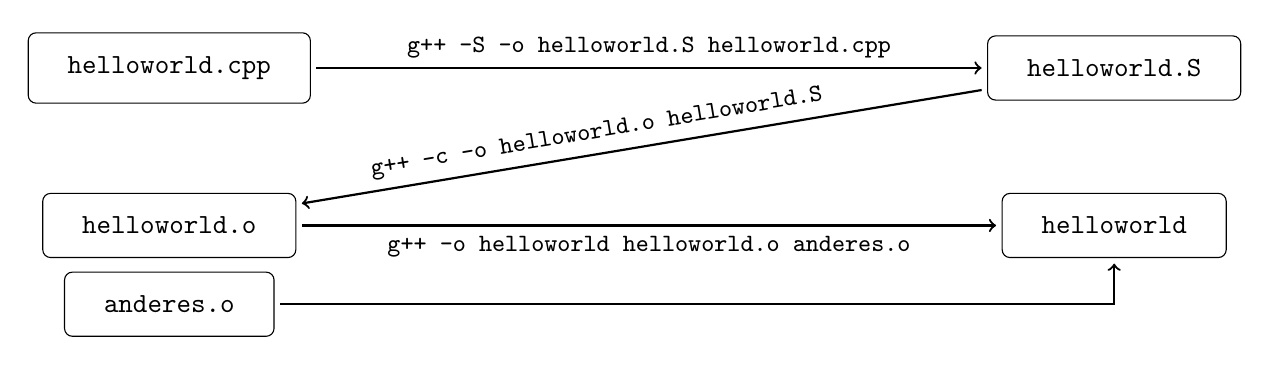
\begin{tikzpicture}
    \tikzstyle{block} = [ shape=rectangle, rounded corners = 0.1cm, draw=black, inner xsep=0.5cm, inner ysep = 0.3cm ];
    \tikzstyle{arr} = [ ->, thick, shorten >= 2pt, shorten <= 2pt ];

    \node (nHelloWorldCpp) [block] {\texttt{helloworld.cpp}};
    \node (nHelloWorldS) [block, right of = nHelloWorldCpp, node distance = 12cm] {\texttt{helloworld.S}};
    \draw [arr] (nHelloWorldCpp) -- (nHelloWorldS) node [midway,above,font=\small] {\texttt{g++ -S -o helloworld.S helloworld.cpp}};
    \node (nHelloWorldO) [block, below of = nHelloWorldCpp, node distance = 2cm] {\texttt{helloworld.o}};
    \draw [arr] (nHelloWorldS) -- (nHelloWorldO) node [pos=0.56,above,sloped,font=\small] {\texttt{g++ -c -o helloworld.o helloworld.S}};
    \node (nAnderesO) [block, below of = nHelloWorldO, node distance = 1cm] {\texttt{anderes.o}};
    \node (nHelloWorld) [block, below of = nHelloWorldS, node distance = 2cm] {\texttt{helloworld}};
    \draw [arr] (nHelloWorldO) -- (nHelloWorld) node [midway,below,font=\small] {\texttt{g++ -o helloworld helloworld.o anderes.o}};
    \draw [arr] (nAnderesO) -| (nHelloWorld) node {};
\end{tikzpicture}

Der bisherige Befehl, den wir zum Kompilieren benutzt haben, ist tatsächlich
nur ein Spezialfall von diesem: Geben wir nämlich auf der Kommandozeile eine
input-Datei an, so rät \texttt{g++} anhand der Dateierweiterung und der
Parameter, was wir damit tun wollen. Er führt dann alle Schritte, um von
unserer input-Datei zu der gewünschten zu kommen automatisch aus, wenn wir also
\texttt{g++ -o helloworld helloworld.cpp} eingeben, dann weiß der Compiler,
dass wir eine ausführbare Datei wünschen (da wir weder \texttt{-c} noch
\texttt{-S} angegeben haben) und dass er dafür kompilieren, assemblieren und
linken muss (da wir ihm eine \texttt{.cpp} Datei gegeben haben). Genauso konnte
er in der vorigen Lektion raten, dass \texttt{g++ -o tictactoe tictactoe.cpp
tictactoe.o} heißt, dass wir eine ausführbare Datei wollen, die aus einem
kompilierten und assemblierten \texttt{tictactoe.cpp} zusammen gelinkt mit
\texttt{tictactoe.o} bestehen soll.

\textbf{Praxis:}
\begin{enumerate}
    \item \texttt{assemble.cpp} enthält ein kleines (ziemlich nutzloses)
        Programm, welches zwei Zahlen addiert und das Ergebnis ausgibt.
        Kompiliert es (nun nur der erste Schritt in dem Diagramm, nicht so, wie
        in den vergangenen Lektionen) und schaut euch das resultierende
        \texttt{.S}-file in einem Editor an. Ihr müsst nicht verstehen,
				was genau hier überall passiert, aber vielleicht findet ihr ja die
				\texttt{main}-Funktion, die Definition der Variablen und die Addition?

        Wir können nun mal Optimierung anschalten -- gebt dazu zusätzlich den
        Parameter \texttt{-O3} direkt nach dem \texttt{g++} an. Schaut euch das
        \texttt{.S}-file nun wieder im Editor an. Was fällt euch
				(im Vergleich zu vorher) auf?
    \item Assembliert eines der im vorigen Schritt erzeugten \texttt{.S} files
        in ein \texttt{.o}-File.
    \item Benennt in einem eurer bisherigen Programme die
        \texttt{main}-Funktion um und versucht, es zu kompilieren (wie in den
        bisherigen Lektionen, also alle Schritte auf einmal). Schaut euch die
        resultierenden Fehlermeldungen an. Wo wird euch der Linkerfehler
        ausgegeben?
    \item Macht die Umbenennung wieder rückgängig und kompiliert das Programm
        erneut -- übergebt aber dieses mal den Quellcode doppelt (also z.B.
        \texttt{g++ -o helloworld helloworld.cpp helloworld.cpp}). Was
        beobachtet ihr? Könnt ihr die Beobachtung erklären?
\end{enumerate}

\inputcpp{assemble.cpp}

\lesson{Tic Tac Toe - Teil 2}

Dies ist die letzte Lektion des ersten Kapitels. In der vorletzten Lektion
haben wir die grobe Struktur eines Tic Tac Toe Spiels implementiert, dafür
haben wir ein paar Funktionen benutzt, die uns gegeben waren. Nun wollen wir
diese Funktionen nachimplementieren („Implementieren“ heißt, dass man eine mehr
oder weniger formale Spezifikation in Programmcode umsetzt). Für eine
Beschreibung, was die Funktionen machen sollen, könnt ihr in der vorletzten
Lektion nachschauen. Damit ihr eure eigene Implementationen testen könnt, haben
wir noch einmal alle Funktionen mit beigefügt. Sie befinden sich in den Dateien
\texttt{frage\_feld\_nummer.o}, \texttt{gebe\_feld\_aus.o} und
\texttt{gewinnerin.o}.

Um eine Funktion zu implementieren, solltet ihr die dazugehörige
\texttt{extern}-Deklaration aus eurer \texttt{tictactoe.cpp} löschen und dann
die Funktion mit dem gleichen Namen (und den gleichen Parametern und
Rückgabetypen) selbst definieren und implementieren. Ihr könnt, wenn ihr z.B.
\texttt{gewinnerin} selbst implementiert habt, euer Programm mit

\texttt{g++ -o tictactoe tictactoe.cpp frage\_feld\_nummer.o gebe\_feld\_aus.o}

kompilieren. Je mehr Funktionen ihr selbst nachimplementiert, desto weniger
gegebene \texttt{.o}-files müsst ihr natürlich angeben.

Es gibt es dieses mal auch keine Nummern für die einzelnen Teile -- sucht euch
doch selbst aus, in welcher Reihenfolge ihr sie bearbeiten wollt, sie ist
ziemlich beliebig. Fangt am Besten mit dem Teil an, der euch am leichtesten
erscheint.

\textbf{Praxis:}
\begin{itemize}
    \item Implementiert \texttt{frage\_feld\_nummer} nach. Ihr solltet darauf
        achten, dass ihr in dieser Funktion auch testen müsst, ob ein gültiges
        Feld eingegeben wurde und ob das angegebene Feld leer ist.
    \item Implementiert \texttt{gebe\_feld\_aus} nach. Ihr könnt euch selbst
        aussuchen, wie ihr die Ausgabe gestalten wollt -- es muss nicht genauso
        aussehen, wie unser Vorschlag. Die
        Wikipedia\footnote{\url{http://en.wikipedia.org/wiki/Box-drawing_character}}
        kann euch z.B. helfen, ein schöneres Feld auszugeben. Fangt am Besten
        mit einer einfachen Ausgabe an und macht sie dann immer „fancier“.
    \item Implementiert \texttt{gewinnerin} nach. Bedenkt, dass ihr alle
        Möglichkeiten testet, auf die ein Gewinn möglich ist -- also 3
        Möglichkeiten, eine Reihe zu bilden, 3 Möglichkeiten, eine Spalte zu
        bilden und 2 Möglichkeiten für Diagonalen. Überlegt euch zunächst, wie
        ihr zwischen Feldnummer (0-8) und Reihen- bzw. Spaltennummer hin- und
        herrechnen könnt. Beachtet auch, dass es ein Unentschieden gibt, wenn
        alle Felder belegt sind, aber keine von beiden Spielerinnen gewonnen
        hat.
\end{itemize}


\pagestyle{empty}

Ihr habt hiermit das erste Kapitel unseres
Programmiervorkurses abgeschlossen. Wir hoffen, ihr hattet dabei Spaß und habt
genug gelernt, um euch gut auf eure erste Programmiervorlesung vorbereitet zu
fühlen.

Rekapitulieren wir noch einmal unsere Eingangs formulierten „Lernziele“, was
wir uns wünschen würden, dass ihr aus diesem Vorkurs mitnehmt:
\begin{itemize}
    \item Ein Computer ist keine schwarze Magie
    \item Eine Konsole ist keine schwarze Magie
    \item Programmieren ist keine schwarze Magie
    \item Ihr wisst, wo ihr anfangt, wenn die Aufgabe ist „schreibt ein
        Programm, das\dots“
    \item Ihr entwickelt Spaß daran, Programmieraufgaben zu lösen
    \item Ihr wisst, was ihr tun könnt, wenn etwas nicht funktioniert
\end{itemize}

Von wie vielen davon habt ihr das Gefühl, sie erreicht zu haben? Wir würden uns
über euer Feedback freuen!


\end{document}
